\documentclass[letterpaper,twocolumn,10pt]{article}

\usepackage[subtle]{savetrees-clean}
\usepackage{usenix}
\usepackage{times}
\usepackage{amsmath}
\usepackage{multirow}
% SOME OF OUR DEFINITIONS
\usepackage[keeplastbox]{flushend}


\usepackage{xspace}
\newcommand{\sys}{Embark\xspace}
\newcommand{\RM}{RM\xspace}

% MBArk
% EMBArk

\usepackage[compact]{titlesec}
\titlespacing*{\section}{0pt}{4pt}{0pt}
\titlespacing*{\subsection}{0pt}{4pt}{0pt}
\titlespacing*{\subsubsection}{0pt}{4pt}{0pt}
\usepackage[small]{caption}
\usepackage{fancyvrb}
\usepackage{listings}
\usepackage[T1]{fontenc}

% more compact than computer modern
\usepackage{times}

% Typewriter Font: Latin Modern Typewriter Proportional
\renewcommand*{\ttdefault}{lmvtt}

\lstset{
  basicstyle=\footnotesize\ttfamily, 
    columns=fullflexible,
    keepspaces=true,
}

\usepackage{subfigure}
\usepackage{ifpdf}
\usepackage[usenames,dvipsnames]{color}
\usepackage[hyphens]{url}
\usepackage[breaklinks, pdfborder={0 0 0}]{hyperref}
\hypersetup{
  backref=true
    bookmarksnumbered,
    colorlinks=true,
    pdfstartview={FitH},
    citecolor={blue},
    linkcolor={blue},
    urlcolor={blue},
    citecolor={blue},
    pdfpagemode={UseOutlines}
}

\usepackage[noend]{algpseudocode}

% edit the comments 
\usepackage{eqparbox}
\renewcommand{\algorithmiccomment}[1]{\eqparbox{COMMENT}{// {\emph #1}}}

\usepackage{enumitem}

\newcommand{\tbd}[1]{}
\newcommand{\ie}{{\it i.e.}}
\newcommand{\eg}{{\it e.g.}}
\newcommand{\etc}{{\it etc.}}


\newcommand{\mypara}[1]{\medskip\noindent{\bf {#1}.}~}
\newcommand{\bpara}[1]{\noindent{\bf {#1}.}~}
\newcommand{\submypara}[1]{\medskip\noindent{\it {#1}.}~}
\newcommand{\chk}{$\checkmark$}
\newcommand{\dsh}{{\bf --}}
\newcommand{\til}{{\bf\large \textasciitilde}}
\usepackage{rotating}

\usepackage{framed}
\FrameSep4pt
\setlength{\topsep}{0pt}

\newcommand{\CTE}{CTE\xspace}
\newcommand{\Name}{APLOMB\xspace}
\newcommand{\Nameplus}{{APLOMB+}\xspace}
\newcommand{\NameArch}{{\sc APLOMB}\xspace}

% ENCRYPTION NOTATION

\newcommand{\ov}[1]{\overline{#1}}

\newcommand{\pmatch}{PrefixMatch}

\newcommand{\plen}{\mathsf{prefix\_len}}
\newcommand{\slen}{\mathsf{suffix\_len}}
\newcommand{\ptlen}{\mathsf{pt\_len}}



\newcommand{\comment}[1]{\hfill {\footnotesize // #1}}

\newcommand{\prefixes}{\mathsf{prefixes}}
\newcommand{\seed}{\mathsf{seed}}

% RESULTS

\newcommand{\generalFHEslowdown}{9\xspace}
\newcommand{\squaregeneralFHEslowdown}{18}
\newcommand{\strawmanslowdown}{10^6}
\newcommand{\setuptime}{414 s}
\newcommand{\strawmansetuptimesslower}{1.8 \cdot 10^3}

\usepackage{enumitem}
\setlist[itemize]{itemsep=0.00cm}
\setlist[itemize]{parsep=0.01cm}
%\setlist[itemize]{parskip=0.01cm}

\newenvironment{myitemize}
{ \begin{itemize}[nolistsep,leftmargin=0.15in]
  \setlength{\itemsep}{0.5pt}
  \setlength{\parskip}{0.9pt}
  \setlength{\parsep}{0.1pt}     }
{ \end{itemize}                  } 

\newcommand{\simplequote}[1]{\\\noindent{\it``{#1}''}\linebreak[3]}
\newcommand{\green}[1]{{\color{ForestGreen}{#1}}}


% our encryption scheme
\newcommand{\bbenc}{DPIEnc\xspace}
\newcommand{\bbdetect}{\sys Detect\xspace}

\newcommand{\RG}{RG\xspace}
\newcommand{\MB}{MB\xspace}

\newcommand{\sslk}{k_{\mathsf{SSL}}}
\newcommand{\bbG}{\mathbb{G}}

\newcommand{\garble}{\mathsf{Garble}}
\newcommand{\eval}{\mathsf{Eval}}
\newcommand{\keygen}{\mathsf{KeyGen}}
\newcommand{\Enc}{\mathsf{Enc}}
\newcommand{\kwenc}{\mathsf{KWEnc}}
\newcommand{\enc}{\Enc}
\newcommand{\Match}{\mathsf{Match}}
\newcommand{\en}{\mathsf{enc}}
\newcommand{\encleft}{\mathsf{EncLeft}}
\newcommand{\encright}{\mathsf{EncRight}}
\newcommand{\match}{\mathsf{Match}}

\newcommand{\sig}{\mathsf{sig}}
\newcommand{\ct}{\mathsf{ct}}
\newcommand{\sno}{\mathsf{serial\_no}}
\newcommand{\dirtyrange}{\mathsf{dirtyrange}}

\renewcommand{\mod}{\mathsf{mod}\xspace}

\newcommand{\low}{\mathsf{low}\xspace}
\newcommand{\high}{\mathsf{high}\xspace}
\newcommand{\prf}{\mathsf{prf}\xspace}
\newcommand{\prefix}{\mathsf{prefix}\xspace}
\newcommand{\IV}{\mathsf{IV}}

\newcommand{\twosnortcom}{67\%}
\newcommand{\twosnortemerge}{42\%}


\newcommand{\SSL}{\mathsf{SSL}}
\newcommand{\rand}{\mathsf{rand}}
\newcommand{\salt}{\mathsf{salt}}

\newcommand{\mf}[1]{ {\fontfamily{cmtt}\selectfont#1}}

\newcommand{\ALGORITHM}[4]{%  name, llabel, intro, \items    
  \let\oldi\labelenumi
    \let\oldii\labelenumii
    \let\oldiii\labelenumiii
    \renewcommand{\labelenumi}{\arabic{enumi}: }
  \renewcommand{\labelenumii}{\arabic{enumi}.\arabic{enumii}: }
  \renewcommand{\labelenumiii}{\arabic{enumi}.\arabic{enumii}.\arabic{enumiii}: }                                     
  \noindent \textbf{#1} \label{#2}
(#3):
  \vspace{0.13\baselineskip}
  \begin{enumerate}[noitemsep,nolistsep]\itemsep=0.1\baselineskip
#4
    \end{enumerate}
  \let\labelenumi\oldi
    \let\labelenumii\oldii
    \let\labelenumiii\oldii  
}

%\newcommand{\subparagraph}{\paragraph}
%\usepackage[compact]{titlesec}

\newcommand{\tickYes}{\checkmark}
\newcommand{\raluca}[1]{{\color{Red}{\bf TODO: }}}
\newcommand{\sr}[1]{{\color{CarnationPink} SR: {#1}}} % :)
\newcommand{\clan}[1]{{\color{SkyBlue} CL: {#1}}} % :)
\newcommand{\qu}[1]{{\color{Magenta}  {\bf Question:} {#1}}} 
\newcommand{\warning}[1]{{\color{Red}{\bf Warning: #1}}}
\newcommand{\todo}[1]{{\color{Red}{\bf TODO: #1 }}}
%\newcommand{\todo}[1]{}
\newcommand{\justine}[1]{{\color{Green}{\bf JS: #1}}}

\newcommand{\aes}{\mathsf{AES}}
\newcommand{\encr}{\mathsf{enc\_r}}


% Compact itemize and enumerate.  Note that they use the same counters and                         
% symbols as the usual itemize and enumerate environments.                                         
\makeatletter
\def\compactify{\itemsep=3pt plus3pt \topsep=3pt plus3pt \partopsep=0pt
  \parsep=0pt \leftmargin=1.3em}
  \let\latexusecounter=\usecounter
  \def\CompactItemize{%                                                                              
    \ifnum \@itemdepth >\thr@@\@toodeep\else
      \advance\@itemdepth\@ne
      \edef\@itemitem{labelitem\romannumeral\the\@itemdepth}%                                        
      \expandafter
      \list
      \csname\@itemitem\endcsname
      {\compactify\def\makelabel##1{\hss\llap{##1}}}%                                              
    \fi}
    \let\endCompactItemize\endlist
    \newenvironment{CompactEnumerate}
{\def\usecounter{\compactify\latexusecounter}
  \begin{enumerate}}
{\end{enumerate}\let\usecounter=\latexusecounter}
\makeatother


% Tweaks
\setlength{\abovecaptionskip}{2pt}
\setlength{\belowcaptionskip}{-15pt}
\frenchspacing
\makeatletter
\g@addto@macro\normalsize{%
  \setlength\abovedisplayskip{2pt}
  \setlength\belowdisplayskip{2pt}
  \setlength\abovedisplayshortskip{2pt}
  \setlength\belowdisplayshortskip{2pt}
}
\makeatother

% Title, authors
\date{}

\title{
  %American capitalization structure.
  \sys: Securely Outsourcing Middleboxes to the Cloud
}

\newcommand{\superscript}[1]{\ensuremath{^{\textrm{#1}}}}
\newcommand{\affila}{\superscript{*}}
\newcommand{\affilb}{\superscript{\dag}}
\newcommand{\affilc}{\superscript{\ddag}}

\author{
  {\rm Chang Lan} \qquad 
  {\rm Justine Sherry} \qquad 
  {\rm Raluca Ada Popa} \qquad 
  {\rm Sylvia Ratnasamy} \qquad 
  {\rm Zhi Liu\affila} \\
  UC Berkeley \qquad \affila Tsinghua University
}

\begin{document}

\maketitle

%!TEX root = mb.tex

\begin{abstract}

It is increasingly common for enterprises and other organizations to outsource network processing -- such as firewalling and caching -- to the cloud, just as they often outsource compute and storage.
However, this poses a threat to enterprise confidentiality because the cloud provider gains access to the organization's traffic.

We design and build \sys, the first system that enables a cloud provider to offer a wide range of middleboxes while maintaining client confidentiality. \sys encrypts the traffic that reaches the cloud and enables the cloud to process the  traffic {\em without decrypting it}.
\sys supports a wide-range of middleboxes such as firewalls, NATs, web proxies, load balancers, intrusion prevention systems, and data exfiltration systems. Our evaluation shows that \sys supports these applications with competitive performance: because \sys makes no modifications to the dataplane for most middleboxes, throughput at most middleboxes is unaffected by our changes.

{\bf TODOS.}
\begin{myitemize}
  \item Add discussion of rules to encryption overview for clarity.
  \item Tone down claims of not changing dataplane -- not changing per-packet algorithms.
  \item Middlebox design/impl section
  \item Add a BlindBox section to Related Work, discuss thoroughly.
  \item New graphs/numbers in Eval
  \item Left Sylvia's draft with comments at home. Re-read for macro-changes I forgot, fix nits.
  \item Mention gateway in intro so no "letdown" effect.
  \item Mention rule optimization in \S 4. 
  \item Uh, are those bandwidth numbers correct????
  \item Clean up related work, tighten/shorten as much as possible.
  \item There are gazillions of missing references and citations.
  \item VERY LAST: cut cut cut cut to length.
\end{myitemize}
\end{abstract}

%!TEX root = mb.tex 

\section{Introduction}\label{sec:intro}

\newcommand{\myspace}{\rule{0pt}{13em}}

\begin{table*}[t]
\centering
\small
{\renewcommand{\arraystretch}{1.8}%
\begin{tabular}{|>{\raggedright}p{3cm}|>{\raggedright}p{8.7cm}|c|c|}
\hline
{\bf Middlebox} & {\bf Functionality} & {\bf Support} & {\bf Scheme} \\ \hline
IP Firewall & 
\parbox {8cm}{
\begin{flalign*}
& (SIP,\ DIP,\ SP,\ DP,\ P) \in (SIP[],\ DIP[],\ SP[],\ DP[],\ P)  \\ 
& \hspace{5mm} \Leftrightarrow  \Enc(SIP,\ DIP,\ SP,\ DP,\ P) \in \Enc(SIP[],\ DIP[],\ SP[],\ DP[],\ P) 
% & \text{To support existing packet classification algorithms {\em unchanged:}} \\
% &    E_1 \le E_2 \Leftrightarrow \Enc(E_1) \le \Enc(E_2), \text{ where } E \text{ is any of } SIP,\ DIP,\ SP,\ DP,\ P
\end{flalign*}
}
& Yes & PrefixMatch \\  \hline 

NAT (NAPT) & 
\parbox {8cm}{
\begin{flalign*}
(SIP_1, SP_1) = (SIP_2, SP_2) &\Leftrightarrow \Enc(SIP_1, SP_1) = \Enc(SIP_2, SP_2) \\
(SIP_1, SP_1) \neq (SIP_2, SP_2) &\Leftrightarrow \Enc(SIP_1, SP_1) \neq \Enc(SIP_2, SP_2) 
\end{flalign*}
}
& Yes & PrefixMatch \\ \hline

L3 Load Balancer (ECMP) &
\parbox {8cm}{
\begin{flalign*}
&(SIP_1, DIP_1, SP_1, DP_1, P_1)\ =\ (SIP_2, DIP_2, SP_2, DP_2, P_2) \\
\Leftrightarrow &\Enc(SIP_1, DIP_1, SP_1, DP_1, P_1)\ =\ \Enc(SIP_2, DIP_2, SP_2, DP_2, P_2) 
\end{flalign*}
}
& Yes & PrefixMatch \\ \hline

L4 Load Balancer &
\parbox {8cm}{
\begin{flalign*}
&(SIP_1, DIP_1, SP_1, DP_1, P_1)\ =\ (SIP_2, DIP_2, SP_2, DP_2, P_2) \\
\Leftrightarrow &\Enc(SIP_1, DIP_1, SP_1, DP_1, P_1)\ =\ \Enc(SIP_2, DIP_2, SP_2, DP_2, P_2) \\
&(SIP_1, DIP_1, SP_1, DP_1, P_1)\ \neq\ (SIP_2, DIP_2, SP_2, DP_2, P_2) \\
\Leftrightarrow &\Enc(SIP_1, DIP_1, SP_1, DP_1, P_1)\ \neq\ \Enc(SIP_2, DIP_2, SP_2, DP_2, P_2) 
\end{flalign*}
}& Yes & PrefixMatch \\ \hline

HTTP Proxy / Cache &
\parbox {8cm}{
\begin{flalign*}
&\text{Request-URI} \in \text{HTTP Header} \\
\Leftrightarrow \quad &\Enc(\text{Request-URI}) \in \Enc(\text{HTTP Header})
\end{flalign*}
} &
Yes & KeywordMatch \\ \hline

Deep Packet Inspection: & & & \\


$\circ$ Parental Filter &
\parbox {8cm}{
\begin{flalign*}
&\text{Request-URI} \in \text{HTTP Header} \\
\Leftrightarrow \quad &\Enc(\text{Request-URI}) \in \Enc(\text{HTTP Header})
\end{flalign*}
} &
Yes & KeywordMatch \\
%
%
$\circ$ Data Exfiltration /  Watermark Detection 
&
$\text{Watermark} \in \text{Stream} \quad \Leftrightarrow \quad \Enc(\text{Watermark}) \in \Enc(\text{Stream})$
 &
Yes & KeywordMatch \\ 
%
%
$\circ$ Intrusion detection
&
$ \text{Keyword} \in \text{Stream} \quad \Leftrightarrow \quad \Enc(\text{Keyword}) \in \Enc(\text{Stream})$
&
Yes & KeywordMatch \\ 
%
%
&
$\text{RegExpMatch(RegExp, Stream)} \ \Leftrightarrow \ \text{RegExpMatch(} \Enc(\text{RegExp}) \text{, } \Enc(\text{Stream}) \text{)}$
&
Partially & KeywordMatch \\

&
Run intrusion detection scripts on traffic stream
 &
No & KeywordMatch \\



 \hline

\end{tabular}
}
\caption[]{Middleboxes supported by \sys. The second column indicates the functionality desired out of the encryption to support these middleboxes correctly. ``Support'' indicates if the middlebox is supported and ``Scheme'' the encryption scheme used.  {\bf Legend:} $\Enc$ denotes encryption, $SIP$ = source IP address, $DIP$ = destination $IP$, $SP$ = source port, $DP$ = destination port, $P$ = protocol,  $E[]$ = a range of $E$. The $(SIP,\ DIP,\ SP,\ DP,\ P)$ thus denotes the tuple describing a connection. \label{tbl:mbreqs}} 
\end{table*}

%\multicolumn{3}{c}}\\

%%%%%%%%%%%%%%%%%%%





\todo{fix the text below in comments}

%A useful piece of text:
%
%Table 1 presents the ``textbook'' functionality of each middlebox supported. This functionality is the basica functionality
%of this box as presented in textbook .. and RFC ...
%Note that some of these middleboxes have become even more complex, supporting additional functionality not present in
%Table 1. Such functionality may or may be supported by \sys. \sys does not support all complex functionalities out there adn we discuss in \S what we do not support. Make clear that the table spells out precisely what we can support and what not. 
%
%In Table XX, we provide the functionality that \sys provides. This covers the functionality of xxx of above and most of the one
%below. Moreover, in eval, we show that we support at least a real middlebox from each of hte examples above. 
%
%------




Middleboxes such as firewalls, NATs, and proxies, have grown to be a vital part of modern networks, but are 
also widely recognized as bringing significant problems including high cost, inflexibility, and complex management.  
These problems have led both research and industry to explore an alternate approach: moving middlebox functionality out of dedicated boxes and into 
software applications that run multiplexed on commodity server hardware~\cite{mb-manifesto,comb,aplomb,opennf,clickos,flowtags,etsi-nfv,domain20,opnfv}.
This approach -- termed Network Function Virtualization (NFV) in industry -- promises many advantages including the cost benefits of commodity infrastructure, 
the efficiencies of statistical multiplexing, and the flexibility of software solutions. 
In a short time, NFV has gained a significant momentum with over 270 industry participants~\cite{etsi-nfv} and a number of emerging product offerings~\cite{brocade,dell,juniper}.

Leveraging the above trend, several efforts are exploring a new model for middlebox deployment in which a third-party offers middlebox processing as a  
\emph{service}.
Such a service may be hosted in a public cloud~\cite{aplomb,zscaler,aryaka} or in private clouds embedded within an ISP 
infrastructure~\cite{domain20, telefonica}.  
This service model allows customers such as enterprises to ``outsource'' middleboxes from their networks entirely, and hence promises many of the known benefits of cloud computing  such as decreased costs and ease of management.%: decreased costs, ease of management, \etc{}.

However, outsourcing middleboxes brings a new challenge: the confidentiality of the traffic. 
Today, in order to process an organization's traffic, the cloud sees the traffic {\em unencrypted}.  This means that the cloud 
now has access to potentially sensitive packet payloads and headers. This is 
worrisome considering the number of documented data breaches by cloud employees or hackers~\cite{PrivacyRecords,databreach}.
Hence, an important question is: can we enable a third party to process traffic for an enterprise, {\em without seeing the enterprise's traffic}?

To address this, we designed and implemented \sys, the first system to allow an enterprise to outsource  a comprehensive set of enterprise middleboxes  to a cloud provider, while keeping its traffic confidential. 
Middleboxes in \sys operate directly over {\it encrypted} traffic. %without decrypting the traffic. 


In recent work, we designed a system called BlindBox to operate on encrypted traffic for a {\em specific} class of middleboxes: Deep Packet Inspection~\cite{blindbox} -- middleboxes that examine only the payload of packets. 
However, BlindBox is far from sufficient for this setting because
 (1) it has restricted functionality that does not support all middleboxes required for outsourcing, and (2) it has prohibitive performance overheads.
 
 Regarding functionality, BlindBox enables equality-based operations on  encrypted payloads of packets, which supports certain DPI devices. However, this excludes middleboxes such as firewalls, proxies, load balancers, NAT,  and those DPI devices that also examine packet headers, because these need the ability to examine packet headers and/or perform range queries. 
 % I added this packet header thing due to NAT
 % even though some of these MB only do exact, the architecture that puts them all together is new
 Achieving such generality provided new challenges to \sys. 
As we discuss below, such middleboxes require a new encryption scheme and, moreover, a system design that supports all middleboxes {\it simultaneously}: for performance, adoption and extensibility, it does not suffice to craft {\it n} different designs to support {\it n} classes of middleboxes. 

 
Regarding performance, BlindBox has a prohibitive setup time of 97s per-connection. 
\sys's setting targets enterprise outsourcing where BlindBox targets end hosts connecting to arbitrary middleboxes. This difference brings \sys new opportunities: it
not only allows us to remove the setup overhead, but also to achieve better deployability and higher security, as we discuss in \S\ref{sec:bbarch}. 

\sys supports a wide range of middleboxes with practical performance. These cover almost all the middleboxes typically outsourced as surveyed in~\cite{aplomb}. 
Table~\ref{tbl:mbreqs} lists these applications. It also lists the desired functionality from encryption in order to support the functionality of this middlebox.  \sys achieves this functionality through a combination of systems and cryptographic innovations, as follows.
   
From a cryptographic perspective, \sys provides a new and fast encryption scheme called PrefixMatch  to enable the provider to perform prefix matching (\eg{}, if an IP address is in the subdomain 56.24.67.0/16) or port range detection (\eg{}, if a port is in the range 1000-2000). Prior to PrefixMatch, there was no mechanism that provided the functionality, performance, and  security needed in our setting. The closest practical encryption schemes are Order-Preserving Encryption (OPE)~\cite{boldyreva:ope,popa:mope,popa:cryptdb}. 
However, these schemes are four orders of magnitude slower than {\it PrefixMatch} making them unusable for our network setting. At the same time, PrefixMatch provides stronger security guarantees than these schemes, which leak unnecessary information to the provider: for every encrypted value, {\em PrefixMatch} reveals only whether the value lies within a range or not, whereas OPE reveals the total ordering among all values.

  From a systems design perspective, one of the key insights behind \sys is to keep packet formats unchanged: an encrypted IP packet is structured just as a normal IP packet, with each field (e.g., source address) containing an encrypted value of that field.
  This strategy ensures that encrypted packets never appear invalid, e.g., to existing network interfaces, forwarding algorithms, and error checking. 
  We choose which encryption scheme to use for each field based on the processing operations applied by typical middleboxes; this results in an encrypted packet that simultaneously supports {\it all} of the wide range of middleboxes we outsource.
  
  Another systems insight is that by {\it combining} standard packet formats with PrefixMatch, \sys can retain compatibility with existing classification algorithms and obtain good performance for middleboxes operating over header fields.
  PrefixMatch ensures that comparisons (such as $\leq$) function normally, hence, a middlebox receiving an encrypted packet can simply perform the normal set of `fast-path' packet processing operations unmodified.
  Importantly, middleboxes can continue to take advantage of highly-efficient packet classification algorithms~\cite{packet_classif} as already implemented, and which are among the more expensive tasks in software middleboxes~\cite{comb, ethan-paper}.
  Furthermore, even software-based NFV deployments make use of some hardware forwarding components, \eg{} NIC multiqueue flow hashing~\cite{nicdocument}, `whitebox' switches~\cite{whitebox}, and error detection in NICs and switches~\cite{nicdocument, ciscov6}; \sys is compatible with all of these.

We implemented and evaluated \sys on EC2. \sys supports all applications typically deployed by outsourcing as surveyed in~\cite{aplomb}.
Further, \sys imposes  negligible throughput overheads at the service provider: for example, a single-core firewall operating over encrypted data achieves 9.8Gbps, equal to the same firewall over unencrypted data.
Our enterprise gateway can tunnel traffic at 9.6 Gbps on a single core;  a single server can easily support 10Gbps for an small-medium enterprise.

%\eat{Relative to BlindBox, \sys is more general. But even when comparing the two directly, \sys (1) has practical performance for deployment, where BlindBox does not: connection session establishment uses standard handshakes and does not have the 97s overhead that BlindBox does; (2) is more secure: \sys can support 79.8\%-88\% of IDS rules without resorting to decryption, where BlindBox can only support 40-67\%; (3) requires no changes to endhosts, where BlindBox requires a new protocol to be supported by each client.} 


\todo{ and where do we put this? In this paper, we consider the functionality of the middlebox to be the one 
described in textbooks and references\todo{add cite}. We note that there exist versions of these middleboxes with different and quite complex functionality that \sys does not support, and we discuss the limitations of \sys in \S\ref{s:limitations}.}


%!TEX root = mb.tex

% 2nd fig/1st fig = 1.12 ratio
\begin{figure*}[t!]
\centering
\subfigure[Enterprise to external site communication]{
  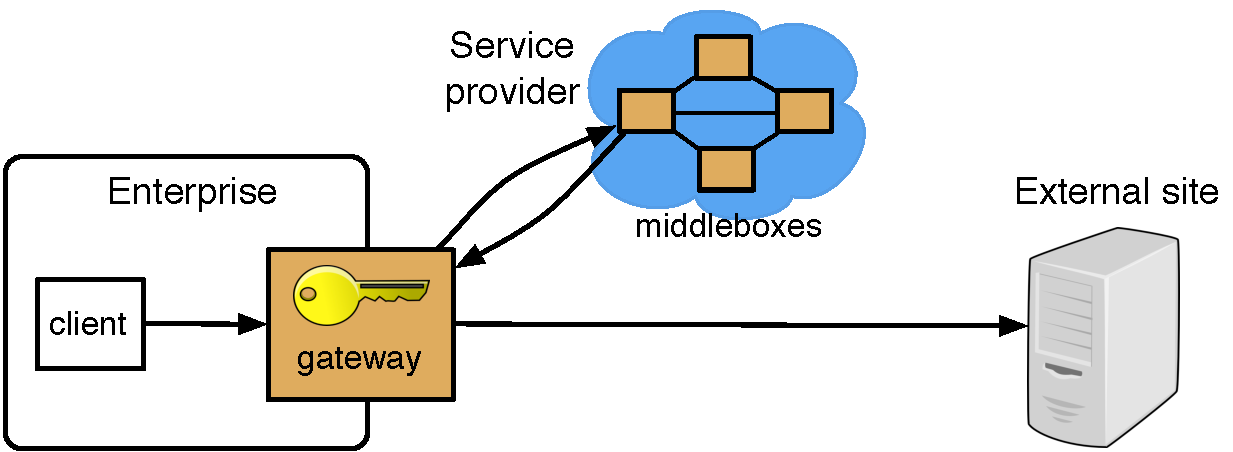
\includegraphics[width=2.8in]{fig/model_1.pdf}
  \label{fig:model1} }
%
\hfill  
\subfigure[Enterprise to enterprise communication]{
   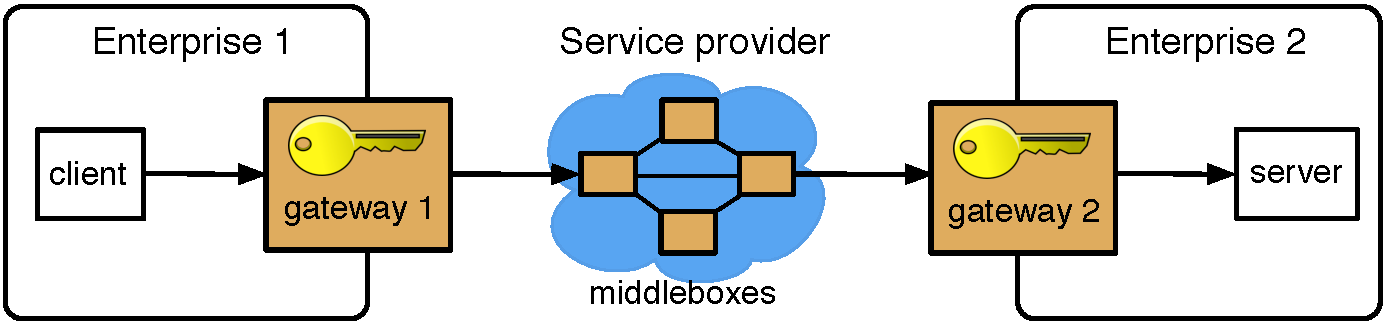
\includegraphics[width=3.2in]{fig/model_2.pdf}
     \label{fig:model2}}
     
     %
\caption{System architecture. Aplomb and NFV system setup with \sys encryption  at the gateway. The arrows indicate traffic from the client to the server; the response traffic follows the reverse direction. \label{fig:sys-overview}}
\end{figure*}




     
\section{Overview}\label{sec:overview}








In this section, we present \sys's architecture, the threat model and applications supported.


% TO CUT REMOVE: just mentino the figures and no need to explain 
\subsection{System Achitecture}

\sys uses the same  architecture as APLOMB, system which redirects an enterprise's traffic to the cloud for middlebox processing~\cite{aplomb}. \sys augments this architecture with confidentiality protection.

The benefits of outsourcing are to delegate the burden of managing and configuring
middleboxes (e.g., upgrading, deciding which vendor to use, monitoring), reduce costs of hardware,
and provide elasticity and fault tolerance; hence \sys should maintain these benefits despite any changes made to to the gateway at the enterprise or middleboxes.
We do not delve further into the details, motivation, and gains of APLOMB's setup, and refer the reader to~\cite{aplomb} for details. 

In the APLOMB setup, there are three parties: enterprise(s), the service provider (SP), and an external site providing
some service. The enterprise runs a gateway (GW) which sends traffic to a middlebox (MB) running in the cloud; in practice this cloud may be either a public cloud service (such as EC2), or an ISP-supported service running at a Central Office (CO).
The service provider -- ISP or cloud-based -- runs a set of middleboxes. 

We illustrate two redirection setups in Fig.~\ref{fig:sys-overview}.  The first setup, in Fig.~\ref{fig:model1},  occurs when the enterprise communicates with an external site: traffic goes to the cloud and back before it is sent out to the Internet. 
It is worth mentioning that APLOMB allows an optimization that saves on bandwidth and latency relative to Fig.~\ref{fig:model1}: the traffic from SP can go directly to the external site and does not have to go back through the gateway. \sys does not allow this optimization fundamentally: the traffic from SP is encrypted and cannot be understood by an external site. We evaluate in \S\ref{sec:eval} what \sys loses by not allowing this optimization. 
Nevertheless, for traffic within the same enterprise, where the key is known by two gateways owned by the same company, we can support this optimization as shown in Fig.~\ref{fig:model2}.




\subsection{Threat Model}

Before defining our threat model precisely, we first provide context and background on the concerns clients have about cloud providers today.

{\bf Context.} 
  Clients adopt cloud services for compute, storage, and increasingly network processing because they the providers are known and trusted to provide good service (at competitive costs). 
  However, while clients trust cloud providers to perform their services correctly, there is increasing concern that cloud providers may access or leak confidential data in the process of providing service.
  Reports in the popular press describe companies selling customer data to marketers~\cite{example}, disgruntled employees snooping or exporting data~\cite{something}, and hackers gaining access to clouds~\cite{somethingelse}.
  The type of threat in this scenario is referred to as an `honest but curious' or `passive'~\cite{goodrich} attacker: a party who is trusted to handle the data and deliver or service it correctly, but who may want to learn more from the data than is strictly necessary or desired.
  Such an attacker differs from a classical, `active' attacker, who seeks to harm the client outright, for example by manipulating data or denying service~\cite{goodrich}.
  This distinction, which based on users concerns today, informs our threat model below. 

{\bf Threat Model.}
The goal of \sys is to protect the privacy of the traffic against an attacker at the service provider  
(cloud employee, or hacker gaining access to cloud machines). 
We consider a strong  attacker, one that has gained access to {\em all the data at SP}.
This includes any traffic and communication SP receives from the 
gateway, any logged information, cloud state, and so on. Nevertheless, we assume that 
SP provides good service and runs middlebox functionality correctly -- but we do not want SP to 
see the traffic in the process of doing so.  

We assume that the gateways are managed by the enterprise and hence trusted; in particular,  they do not leak information.


Some middlebox functionalities (such as intrusion or exfiltration detection) have a threat model
of their own about the client and the server. For example, intrusion detection assumes that 
the client or the server could misbehave, but at most one of them misbehaves~\cite{Bro}.  
%(indeed, if both misbehave, they can send attack traffic to each other encrypted with a shared symmetric key and fundamentally
%no one can detect such an attack).  
We preserve these threat models unchanged. These applications rely
on the middlebox to detect attacks in these threat models. Since we assume the middlebox executes
its functions correctly and \sys preserves the functionality of these middleboxes, 
these threat models are irrelevant to the protocols in \sys, and we will not discuss them again. 

\textbf{In comparison to BlindBox and APLOMB.}
APLOMB~\cite{aplomb} assumes that the provider is fully trusted with client data; \sys's threat model allows for a passive attacker with access to the clients' data at the cloud.
The differences between BlindBox~\cite{blindbox} and \sys are threefold:

%
\noindent(1) With BlindBox, the middlebox and client are unknown to each other; the middlebox wishes to {\it enforce} a policy over the client's traffic, and the client is not allowed to observe the rules being enforced. With \sys, the policy imposed over a clients traffic is a policy the client {\it wishes to have enforced}. 
Some rules may come from the client itself -- such as exfiltration policies -- while others may come from a trusted rule provider such as McAfee or Symantec, as in BlindBox. We discuss how rules are generated and exchanged between the gateway and the cloud in \S\ref{sec:gateway}.
An additional consequence of this shift -- that the client now desires that the policy be enforced properly -- is that BlindBox requires some validation that the client has not attempted to evade proper encryption, whereas our client is trusted to faithfully operate the protocol.
%

\noindent(2) Under \sys, the gateway is trusted by all end hosts at the enterprise network; it performs encryption on their behalf. This gives \sys deployability benefits relative to BlindBox -- only one gateway needs to be upgraded to support the new protocol, not every end host on the network. It also gives performance benefits: where BlindBox incurs a costly setup operation of around 97s for every connection, this setup occurs {\it once} at the gateway under \sys to establish a persistent connection shared by all end hosts. This is only possible because the gateway exists as a trusted intermediary in the network.

\noindent(3) BlindBox provides privacy guarantees comparable to SSL: a middlebox will observe packet headers, but not payload contents. \sys provides stronger privacy coverage, comparable to IPSec in that it obscures all packet headers as well as payloads.

%
%
\subsection{Encryption Overview}
\eat{
\begin{figure}[t!]
\centering
  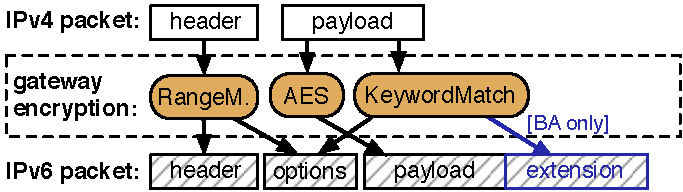
\includegraphics[width=3.0in]{fig/packet.pdf}
\caption{Packet encryption at the gateway. Patterned squares indicate encrypted data. Only for DPI  middleboxes,  KeywordMatch produces additional encrypted data. \justine{Change fig to say DPI not BA}  \label{fig:packet}}
\end{figure}
}

\begin{figure*}[t!]
\centering
  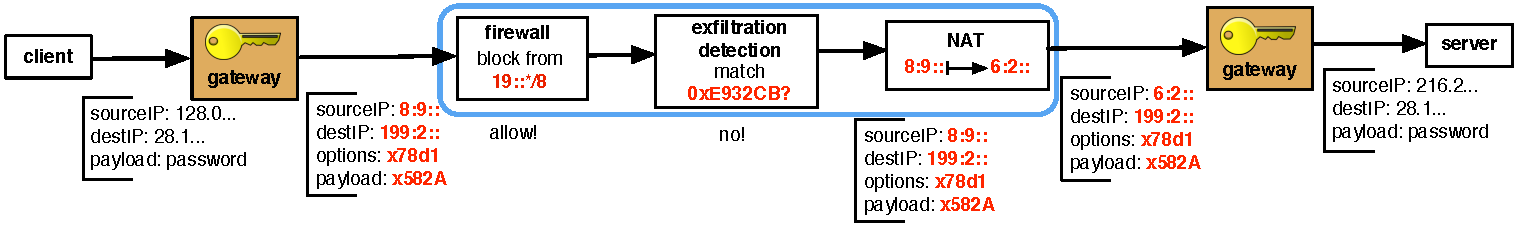
\includegraphics[width=6.7in]{fig/packetpath.pdf}
\caption{Example of packet flow through a few middleboxes. Red in bold indicates encrypted data. \label{fig:packetflow}}
\end{figure*}



To protect privacy , \sys encrypts all traffic passing through the service provider (SP).
\sys encrypts IP addresses, ports, and the payload of the packet.
As in Fig.~\ref{fig:sys-overview}, the gateway has a secret key $k$; in the setup with two gateways, they share
the same secret key. The gateway encrypts all traffic going to the service provider using \sys's encryption schemes.
The middleboxes at SP process {\em encrypted traffic} using \sys's protocols. 
To perform detection, the service provider uses a set of {\it encrypted rules} that allow it to perform comparisons against the encrypted values it observes in the traffic.
After the processing, the middleboxes
will produce encrypted traffic which SP sends back to the gateway. The gateway decrypts the traffic using the key $k$.

Throughout this process, middleboxes at SP handle only encrypted traffic and never access the decryption key. This ensures
that an attacker that steals all the data from SP will  see only encrypted traffic, which protects the privacy of the 
traffic. 
On top of \sys's encryption, the gateway can use a secure tunneling protocol, such as SSL or IPSec to secure the communication to SP.

\begin{table}
\centering
\small
\hspace{-2pt}
\begin{tabular}{l|l|p{.45in}|p{.45in}|p{.45in}}
&{\bf MB}&{\bf TCP/IP Header}&{\bf HTTP Headers}&{\bf Byte Stream}\\

\hline

\parbox[t]{1mm}{\multirow{3}{*}{\rotatebox[origin=c]{90}{Header}}}
&IP Firewall&Range&n/a&n/a\\
&L4 LB&Range&n/a&n/a\\
&NAT&Exact&n/a&n/a\\
\hline


\parbox[t]{1mm}{\multirow{2}{*}{\rotatebox[origin=c]{90}{DPI}}}
&IPS&Range&Exact&Exact\\
&Exfiltration&Range&Exact&Exact\\
\hline

\parbox[t]{1mm}{\multirow{3}{*}{\rotatebox[origin=c]{90}{HTTP}}}
&Proxy&Exact&Exact&n/a\\
&Parent Filter&n/a&Exact&n/a\\
&L7 LB&Exact&Exact&n/a\\
\hline
*&VPN&n/a&n/a&n/a\\

\end{tabular}
\caption[]{Middleboxes supported by \sys and categorized as Header, DPI, or HTTP middleboxes depending on what fields they access. Middleboxes are also labeled whether they perform `exact match' comparisons against rules, or `range match' comparisons against rules.\label{tbl:mbreqs}}

\end{table}



\noindent\textbf{Packet encryption}
Recall that the provider holds a set of encrypted rules at the middleboxes which it uses to operate over the client's encrypted traffic.
\sys uses three encryption schemes to protect data privacy while allowing comparison against encrypted rules at the cloud: 
\begin{myitemize}
\item Traditional AES: provides strong security and no computational capabilities)
\item KeywordMatch:  allows the provider to detect if an encrypted value in the packet is equal to an encrypted rule value
\item RangeMatch: allows the provider to detect whether or not an encrypted value lies in a range of rule values -- e.g. addresses in 128.0.0.0/24 or ports between 80-96.
\end{myitemize}
We discuss these cryptographic algorithm in \S\ref{sec:buildingblocks}.

The key idea behind \sys is to encrypt {\it each field} of a packet using the appropriate encryption algorithm such that middleboxes can process each field of data as if it were not encrypted. 
Plaintext packets are encrypted, field-by-field, to generate a new IPv6 packet that is processed at the cloud.
For example, an encrypted IPv6 packet will contain a source address that is an encryption of the original packet's source address using RangeMatch. This allows, e.g., a firewall to check whether the packet's source belongs to a prefix known to be controlled by a botnet -- but without learning what the actual source IP address is.
We use IPv6 at the cloud because our RangeMatch scheme requires 128 bits to encode an encrypted IP address -- and because we expect more and more service providers to be moving to IPv6 by default in the future.
This is a trivial requirement to impose, as it is easy to convert from IPv4 to IPv6 (and back) at the gateway~\cite{6to4,4to6}; clients may continue using IPv4 and the tunnel connecting the client to the provider may be either v4 or v6.

We choose which encryption scheme is appropriate for each field based on a high level classification of middlebox capabilities.
Table~\ref{tbl:mbreqs} shows a list of all middleboxes supported by typical outsourcing deployments~\cite{aplomb} and their processing requirements.
We classify these middleboxes as operating only over packet headers, operating only over packet headers and HTTP headers, or operating over all data including arbitrary fields in the connection bytestream (DPI).
We revisit these middleboxes in detail in \S\ref{sec:mbs}.


{\bf Example.} Fig.~\ref{fig:packetflow} shows the end-to-end flow of a packet through three example middleboxes in the cloud, each middlebox operating over an encrypted field.  
First,  the gateway encrypts the packet as explained above. The packet passes through the firewall which tries to match the encrypted information from the header against its encrypted rule, and decides to allow the packet. Next, the exfiltration device checks for any suspicious (encrypted) strings on the extension of the packet's payload, and not finding any, it allows the packet  to continue to the NAT. The NAT maps the source IP address to a different IP address. Back at the gateway, the gateway decrypts the packet. 




%!TEX root = mb.tex



\section{Cryptographic Building Blocks}
\label{sec:buildingblocks}

In this section we present the building blocks \sys relies on.
Symmetric-key encryption (based on AES) is well known, and we do not discuss it here. Instead, we briefly discuss KeywordMatch (introduced by~\cite{blindbox}, to which we refer the reader for details) and more extensively discuss PrefixMatch, a new cryptographic scheme we designed for this setting.
When describing these schemes we refer to the encryptor as the gateway whose secret key is $k$ and to the entity computing on the encrypted data as the service provider (SP).


\subsection{KeywordMatch}\label{s:kwmatch}


KeywordMatch allows detecting if an encrypted keyword matches an encrypted data item by equality.
For example, given an encryption of the keyword ``malicious'', and a list of encrypted strings  [$\Enc$(``alice''), $\Enc$(``malicious''), $\Enc$(``alice'')], SP can  detect that the keyword matches the second string. 
For  this, we use a searchable encryption scheme~\cite{song:search, blindbox}.
Using this scheme, the gateway can encrypt a value $v$ into $\enc(v)$ and a rule $r$ into $\encr$ and SP can detect if there is a match between $v$ and $r$. 
 The security of searchable encryption is well studied~\cite{song:search, blindbox}: at a high level,  given a list of encrypted strings, and an encrypted keyword, SP does not learn anything about the encrypted strings, other than which strings match the keyword. 
 The encryption of the strings is {\em randomized}, so it does not leak whether two encrypted strings are equal to each other, unless, of course, they both match the encrypted keyword. 
  We use the technique from~\cite{blindbox} and hence do not elaborate on it.

%!TEX root = mb.tex

%\section{Building block: Range match}
%An important operation over an encrypted packet is to determine if an encrypted field in the packet falls in an encrypted range.
%We will use the firewall as an example. 
%Consider the following firewall rule:
%
%Constructing an encryption scheme that allows checking if an encrypted value is in an encrypted range, has been a challenge in the applied cryptography community. The reason is that ..
%
%\begin{itemize}
%\item preserve the order between Encryptd values
%\item candidate: OPE
%\item candidate: mOPE
%\item So none of the existing schemes are satisfactory. A new scheme \RM.
%\end{itemize}
%
%\RM applies to cases when we know an upper bound on the values encrypted with OPE and this is a small number of values (say, less than 10,000).
%
%The small number of values permits us to improve in two ways over mOPE [1]
%No more interaction. We store the tree in mOPE on the gateway (client) side, which means that the gateway can compute a new encryption by itself without help from service provider. The storage at the gateway will remain small.
%Rare updates to ciphertexts. We can space out the ciphertexts of the values encrypted sufficiently. 
%
%This also enjoys a stronger security than OPE! It leaks less than order.
%The reason is that, the server does not learn the order between the values in packets, and only whether they map between two values in the rules. 
%
%this one is new
%
%discuss 
%
%would be good to explain the challenge from the 
%
%\todo{a more interesting name to the scheme}
%
%prefix gets mapped into interval, at most a certain number
%
%talk about building certain data structures that all works the same
%
%firewall need not change 

\subsection{PrefixMatch} \label{sec:range}


Many middleboxes perform detection over {\it prefixes} or {\it ranges} of  IP addresses or port numbers  (i.e. packet classification). To illustrate PrefixMatch, we use IP addresses (IPv6), but the scheme works with 
ports and other value domains too.
For example, a network administrator might wish to block access to all servers hosted by MIT, in which case the administrator would block access to the prefix 0::ffff:18.0.0.0/104, \ie{}, 0::ffff:18.0.0.0/104--0::ffff:18.255.255.255/104. 
PrefixMatch enables a middlebox to tell whether an encrypted IP address $v$ lies in an encrypted range $[s_1, e_1]$, where $s_1$ = 0::ffff:18.0.0.0/104 and $e_1$ = 0::ffff:18.255.255.255/104; however, the middlebox does not learn the values of $v$, $s_1$, or $e_1$. Unlike KeywordMatch, PrefixMatch is a new scheme we designed specifically for our setting.


One might ask whether PrefixMatch is necessary, or one can instead employ KeywordMatch using the same expansion technique we used for some (but not all) regexps in \S\ref{sec:bbarch}. 
To detect whether an IP address is in a range, one could enumerate all IP addresses in that range and perform an equality check. However, the overhead of using this technique for common network ranges such as firewall rules is prohibitive.
For our own department network, doing so would convert our IPv6 and IPv4 firewall rule set of only 97 range-based rules to $2^{238}$ exact-match  rules; looking only at IPv4 rules would still lead to 38M exact-match rules.
Hence, for efficiency, we need a scheme for matching ranges.

\mypara{Requirements}
%
There are a few requirements \sys needs from PrefixMatch.
%
First, PrefixMatch must allow for direct order comparison (i.e., using $\leq$/$\geq$) between an encrypted value $\Enc(v)$ and the encrypted endpoints $\ov{s}_1$ and $\ov{e}_1$ of a range, $[s_1, e_1]$. This allows existing packet classification algorithms, such as tries, area-based quadtrees, FIS-trees, or hardware-based algorithms~\cite{packet_classif}, 
 to run unchanged. 

Second, to support the functionality of NAT in Table~\ref{tbl:mbreqs}, $\Enc(v)$ should be {\em deterministic} within a flow. Recall that a flow is a 5-tuple of source IP and port, destination IP and port, and protocol. Moreover, the encryption corresponding to two pairs (IP$_1$, port$_1$) and  (IP$_2$, port$_2$) that are different should be different.

Third, for security, we require that nothing leaks about the values $v$ encrypted other than what is needed by the functionality above. Note that \sys does not need order comparison between $\Enc(v_1)$ and $\Enc(v_2)$; hence, PrefixMatch does not leak such order information.  PrefixMatch also provides protection for the endpoints of ranges: SP should not learn their values, and SP should not learn the ordering of the intervals. 
 Further, note that the NAT does not require that $\Enc(v)$ be deterministic across flows; hence, PrefixMatch hides whether two IP addresses encrypted as part of different flows are equal or not. In other words, PrefixMatch is randomized across flows.
 


In terms of performance, both encryption (performed at the gateway) and detection (performed at the middlebox) should be practical for typical middlebox line rates.
Our PrefixMatch encrypts in $< 0.5\mu$s per value (we evaluate in \S\ref{sec:eval}), and the detection is the same as regular middleboxes based on the $\leq$/$\geq$ operators.

 To the best of our knowledge, PrefixMatch is the only encryption scheme that achieves these security guarantees and is practical for our setting.
 Order-preserving encryption such as BCLO~\cite{boldyreva:ope} or mOPE~\cite{popa:mope} can provide the same and more functionality than PrefixMatch. In comparison, PrefixMatch provides significantly stronger security by not leaking the order of values encrypted, and achieves four orders of magnitude higher performance  (as we show in \S\ref{sec:eval}).






\mypara{Functionality}
PrefixMatch encrypts a set of ranges or prefixes $P_1, \dots, P_n$ into a set of encrypted prefixes. For each $P_i$, there is one or more corresponding encrypted prefixes: $\ov{P}_{i,1} \dots, \ov{P}_{i, n_i}$.  Additionally, \pmatch{} encrypts a value $v$ into an encrypted value $\Enc(v)$. These encryptions have the  property that, for all $i$,  
%
\[  v \in P_i  \Leftrightarrow \Enc(v) \in \ov{P}_{i, 1} \cup \dots \cup \ov{P}_{i, n_i}. \]
%
In other words, the encryption preserves prefix matching.



For example, suppose that encrypting $P$ =  0::ffff:18.0.0.0/104 results in one encrypted prefix $\ov{P}$ = 1234::/16, encrypting $v_1$ = 0::ffff:18.0.0.2 results in  
 $\ov{v_1}$ = 1234:db80:85a3:0:0:8a2e:37a0:7334, and encrypting $v_2$ = 0::ffff:19.0.0.1 results in 
$\ov{v_2}$ = dc2a:108f:1e16:992e:a53b:43a3:00bb:d2c2. We can see that $\ov{v_1} \in \ov{P}$ and $\ov{v_2} \notin \ov{P}$. 




\subsubsection{Scheme} 
\label{sec:rmscheme}

\begin{figure}[t]
  \centering
  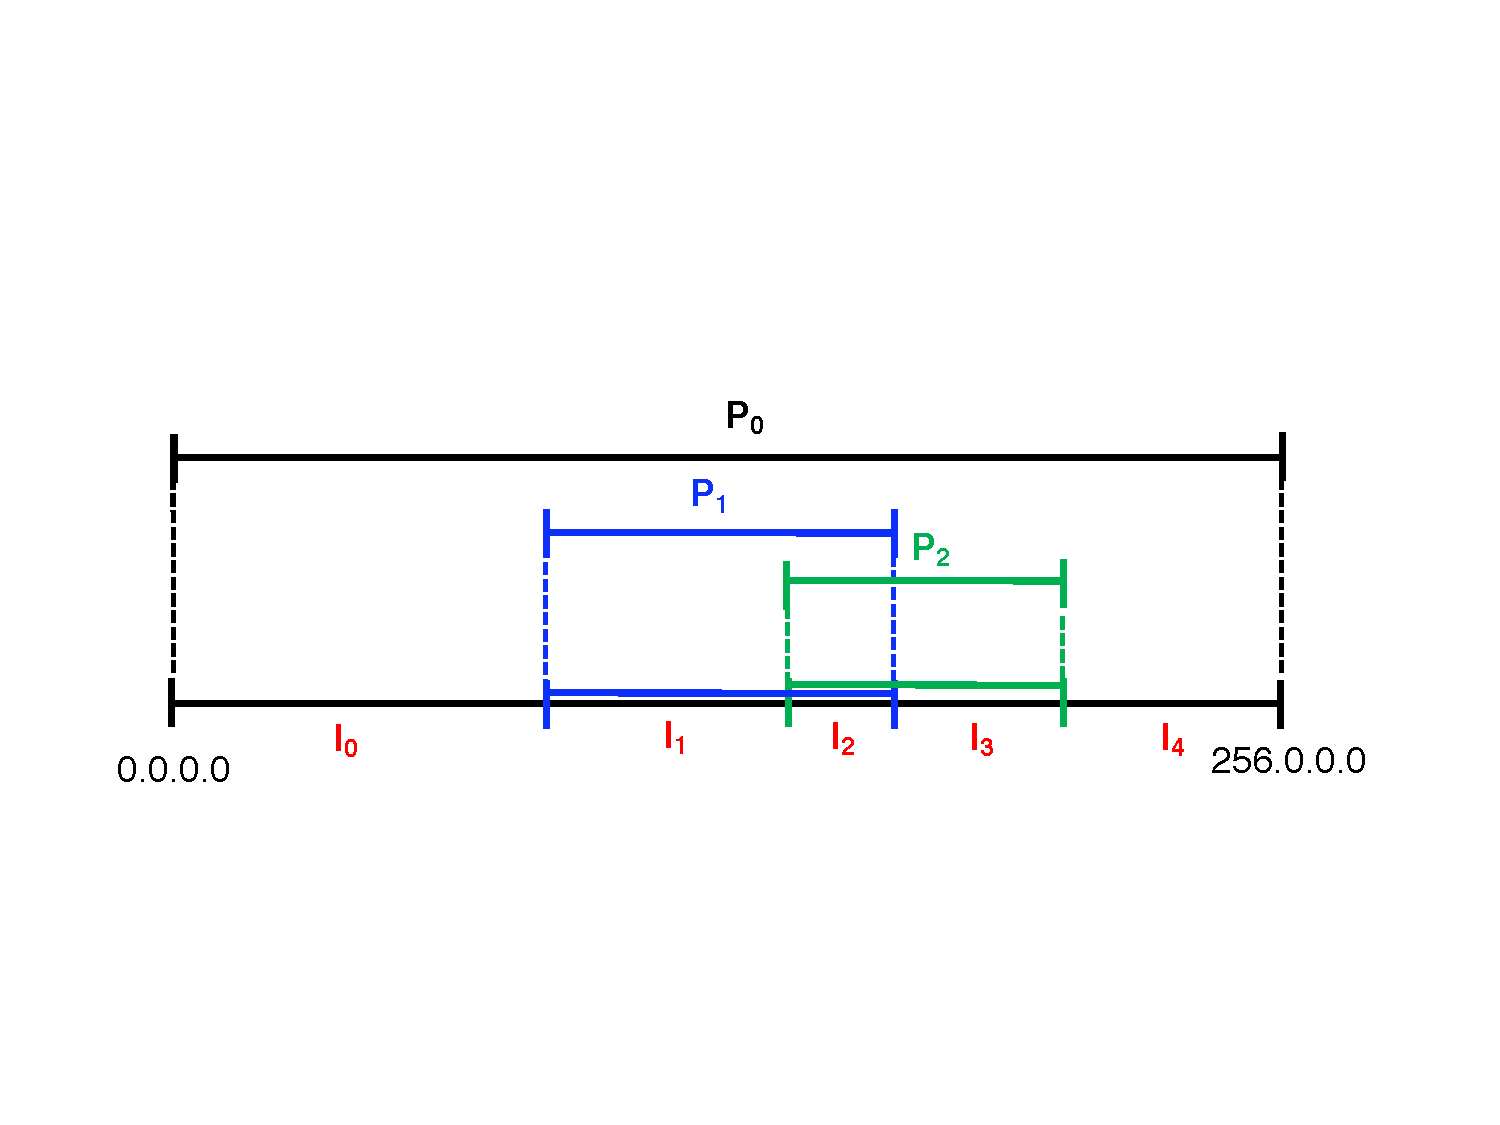
\includegraphics[width=3in]{fig/rangeopts3.pdf}
  \caption[]{Example of prefix encryption with PrefixMatch.\label{fig:rangeopts3}}
\end{figure}

We now explain how PrefixMatch works.  PrefixMatch provides two algorithms: EncryptPrefixes to encrypt prefixes/ranges and EncryptValue to encrypt a value $v$.



\mypara{Prefixes Encryption} \pmatch{} takes as input a set of prefixes or ranges $P_1 = [s_1, e_1], \dots, P_n=[s_n, e_n]$, 
whose endpoints have size $\len$ bits. \pmatch{} encrypts each prefix  into a set of encrypted prefixes: these prefixes are $\plen$ bits long. As we discuss below, the choice of $\plen$ depends on the maximum number of prefixes to be encrypted. For example,  $\plen = 16$ suffices for a typical firewall rule set.

Consider all the endpoints $s_i$ and $e_i$ laid out on an axis in increasing order as in Fig.~\ref{fig:rangeopts3}.
Add on this axis the endpoints of $P_0$, the smallest and largest possible values, $0$ and $2^{\ptlen}-1$.
Consider all the intervals formed by each consecutive pair of such endpoints. 

For example, consider Fig.~\ref{fig:rangeopts3}.  There are two prefixes to encrypt: $P_1$ and $P_2$. PrefixMatch computes intervals $I_0, \dots, I_4$.

PrefixMatch now assigns an encrypted prefix to each interval. Note that each interval belongs to a set of prefixes. Let $\prefixes(I)$ denote the prefix of interval $I$. For example, $\prefixes(I_2) = \{P_0, P_1, P_2\}$. The encrypted prefix is simply a {\em random} number of size $\plen$. Each interval gets a different random value, except for the intervals that belong to the same prefixes. For example, in Fig.~\ref{fig:rangeopts3}, intervals $I_0$ and $I_4$ receive the same random number.

When an interval overlaps partially with another interval, it will have more than one encrypted prefix. For example, consider that $\plen = 16$, $I_1$ was assigned a random number of $0x123c$ and $I_2$ of $0xabcc$. The encryption of the prefix $P_1$ in Fig.~\ref{fig:rangeopts3} will be the pair ($123c::/16$, $abcc::/16$).

Since the encryption is a random prefix, the encryption does not reveal the original prefix. Moreover, the fact that intervals pertaining to the same set of prefixes receive the same encrypted number hides where an encrypted value matches, as we discuss below. For example, for an IP address $v$ that does not match either $P_1$ or $P_2$, the cloud provider will not learn whether it matches to the left or right of $P_1$ and $P_2$ because $I_0$ and $I_4$ receive the same encryption. The only information it learns about $v$ is that $v$ does not match either $P_1$ or $P_2$. 

We now present the EncryptPrefixes procedure, which works the same for prefixes or ranges.



\begin{framed}
\ALGORITHM{EncryptPrefixes}{proc:enc_prefixes}{$P_1$, $\dots$, $P_n$, $\plen$, $\ptlen$, $\slen$}{
\item Let $s_i$ and $e_i$ be the endpoints of $P_i$. \comment{$P_i = [s_i, e_i]$}
	\item Assign $P_0 \gets [0, 2^{\ptlen}-1]$
	\item Sort all endpoints in increasing order
	\item  Construct intervals $I_0, \dots, I_m$ from each pair of consecutive endpoints. Multiple equal endpoints form a unit interval. For each interval $I_i$, compute $\prefixes(I_i)$, the list of prefixes $P_{1}, \dots, P_{m_i}$ that contain   $I_i$. 
	\item Assign a distinct random value of size $\plen$ to each of $\ov{I_0}, \dots, \ov{I_m}$  
	\item For all $i, j$ with $i<j$ if the prefixes containing $I_i$ and $I_j$ are the same, set $\ov{I_j} \gets \ov{I_i}$
	\item The encryption of $P_i$ is $\ov{P_i} = \{\ov{I_j}/\plen, I_j \in \prefixes(P_i) \}$. The encrypted prefixes are output sorted by value (as a means of randomization).
	\item Output $\ov{P_1}, \dots,\ \ov{P_n}$ and the {\em interval map} [$I_i \rightarrow \ov{I_i}$] 
}
\end{framed}

\mypara{Value Encryption}
To encrypt a value $v$, PrefixMatch locates the one interval $I$ such that $v \in I$. $\ov{I}$ becomes the prefix of the encryption of $v$. This ensures that the encrypted $v$, $\ov{v}$, matches $\ov{I}/\plen$. The suffix of $v$ is chosen at random. The only requirement is that it is deterministic. 
Hence, the suffix is chosen based on a pseudorandom function that $\prf^{\slen}$ seeded in a given seed  $\seed$.  



For example, if $v$ is 127.0.0.1 (0::ffff:127.0.0.1), and the assigned prefix for the matched interval is $abcd::/16$, a possible encryption given the ranges encrypted above is $Enc(v) = abcd:ef01:2345:6789:abcd:ef01:2345:6789$. Note that the ecryption does not retain any information about $v$ other than the interval it matches in. In particular, two values $v_1$ and $v_2$ that match the same interval, their order can be arbitrary. Thus, PrefixMatch does not reveal order.

\begin{framed}
\ALGORITHM{EncryptValue}{proc:enc_value}{$\seed$, $v$, $\slen$, interval map}{
\item Run binary search on interval map to locate the interval $I$ such that $v \in I$.
\item Lookup $\ov{I}$ in the interval map.
\item Output 
\begin{equation}
\Enc(v) = \ov{I} \Vert \prf_\seed^\slen(v)
\end{equation}
}
\end{framed}

\todo{introduce suffix len}

%\begin{figure}
%  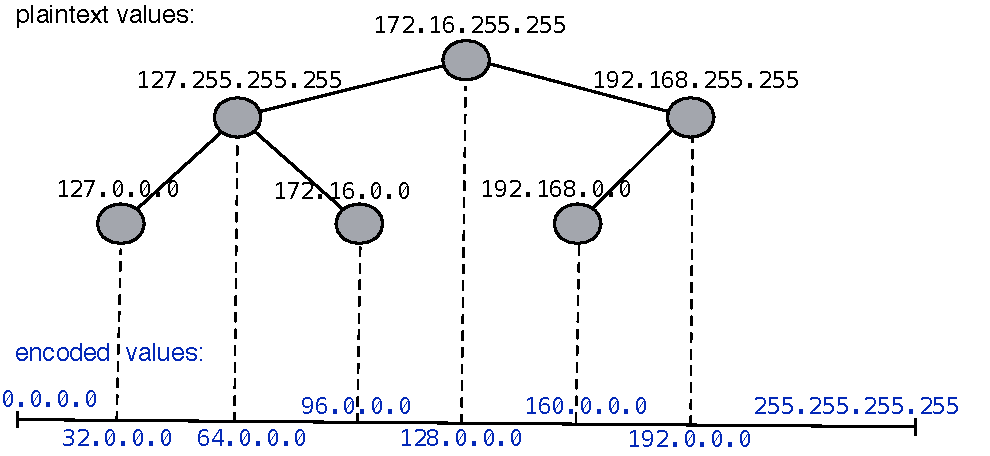
\includegraphics[width=3.25in]{fig/tree}
%  \caption{\label{fig:tree} PrefixMatch tree. The values of nodes in the tree are the %unencrypted IP addresses, and the blue values on the horizontal axis are their encryptions. }
%\end{figure}

\mypara{Comparing encrypted values against rules}
Determining if an encrypted value matches an encrypted prefix is straightforward: the encryption preserves the prefix.
Hence, a regular packet classification can be run at the firewall with no modification. Comparing different encrypted values for order that match the same prefix is meaningless, and returns a random value.


\todo{attention, there is also the determinism that leaks}

\subsubsection{Security Guarantees}

\pmatch{} hides the endpoints of ranges or the prefixes encrypted with EncryptPrefixes and it does not reveal the values encrypted with EncryptValue. \pmatch{} reveals only matching information between values and prefixes to enable functionality at the cloud provider.  For every subset of prefixes out of $P_1, \dots, P_m$, the cloud provider learns if these overlap and whether an encrypted value $v$ matches them. In particular, the cloud provider does not learn the order of encrypted values $\Enc(v)$ or the order of the prefixes. Hence, PrefixMatch is significantly more secure than order-preserving encryption.

%
Since the encryption is seeded in a per-connection identifier, correlation attacks between different flows are not possible. 
In particular, even though EncryptValue is deterministic, the encryption of the same IP address in different flows will be different because the seed differs per flow.
\todo{the above sentence needs some context}

We formalize and prove the security guarantees of \pmatch{} in our extended paper. 

\subsubsection{Implementing PrefixMatch in the Gateway}
\label{sec:tree}

\todo{THIS  SUBSECTION IS WORK IN PROGRESS}
\todo{give syntax somewhere?}



\todo{make clear that the same key is used for equality matching, somewhere in the gateway}
\todo{we do 4 to 6 translation}

To encrypt a value with EncryptValue, we seed $\prf$ in $\seed$, a function of both the key and hash of the tuple being encrypted ($\seed = \prf_k(\text{(u, v)})$). Note that, in the system setup with two gateways, the gateways generate the same encryption because they share $k$.  

The scheme supports NATs -- which require that every time a value for the same connection is encrypted, it returns the same value. It generates a random encryption using a deterministic function. 

When encrypting IP addresses, we do not want two different IP addresses to map to the same encryption (which would break the NAT). Fortunately, the probability that two IP addresses get assigned to the same encryption is negligibly low for IPv6.  The reason is that each interval of prefixes is large because we distributed the endpoints evenly and because there is a small number of such endpoints in a realistic setting (e.g., a firewall has less than 100,000 rules). Suppose we have $n$ distinct rules, $m$ flows and a $w$-bit space, with the assumption of uniformly distributed flows, the probability of getting collision is approximately 

\begin{equation}
1 - e^\frac{-m^2 (2n+1)}{2^{w+1}}
\end{equation}

\todo{discuss how the gateway gives the seed -- is the choice of seed outside of the prefixmatch alg or inside?}
\todo{discuss security of ports clearly}

Therefore, if $w=128$ (which is the case when we use IPv6), the probability is negligible in a normal setting. When encrypting ports, it is possible to get collisions since the port field is only 16-bit. However, this will not cause problem as long as the IP address does not collide, because NATs (and other middleboxes that require injectivity) considers both IP addresses and ports.

\todo{make clear that it is seeded in this so IPs do not collide}


\todo{need to discuss how the firewall puts prefix match in the prefix form, and adds /*}

\todo{remark for perfect security and tradeoff with work at the gateway}
\todo{does each rule become multiple rules?? explain who FW does with this, explain how many there are, need eval of this}
\todo{then in func you also need to clarfiy that it becomes more than one; this will leak about the prefixes what intersections they have!! even without fields matching}
\todo{and what does the firewall do?}


\todo{ I wonder how much of this section actually needs to move to the gateway section}

\todo{ need to discuss how the gateway chooses k for the encryptvalue -- the seed}

\noindent \textbf{Updating ranges.}
Adding a new range or removing an existing range would affect the intervals it covers. Therefore, in the worst case $O(N)$ rules needs to be updated. 

\todo{ and it has to be clear that to encrypt firewall rules at the gateway using the Prefix match, you need to go through each part of the rule and encrypt that; 
The gateway will use an instance of PrefixMatch for every field, destination IP, etc.
}
\todo{and need to discuss the prefix part}

\todo{need to discuss the fact that they blowup here}


The gateway stores the intervals and the mapping from intervals to prefixes for each field of the rules, and it maintains no state per IP address encrypted or per connection.

The gateway can use the following functions. EncryptRules encrypts the initial rules. EncryptTuple encrypts packet header fields which are represented as a tuple; it requires identifying the interval $I$ for each field. We can compute $I$ efficiently in logarithmic time by doing a binary search. 




% We now describe the procedure for AddRange which adds an interval (deleting an interval is similar). These procedures modify the state at the gateway. To add a range [$s$, $e$], the gateway inserts these values in the tree. If the tree needs to be rebalanced, for each endpoint that changed location in the tree, the gateway records the old and new encrypted value based on the tree in a list $L$. Note that  the number of endpoints that change encryption is $O(\log n)$ amortized worst-case. The gateway then computes the encryption of $s$ and $e$ based on their location in the tree. It sends to SP $\enc(s)$ and $\enc(e)$ along with $L$. 

%Besides the interval added or deleted, a small number
%of other intervals may be moved -- at worst, $O(\log n)$. 
%For these, the algorithm returns the old and new encryption of the interval. 

%
%\begin{framed}
%\begin{algorithmic}[1]
%
%\Procedure{AddRange}{$[s, e]$}
%  \State Insert $s$ and $e$ into the scapegoat tree. If $s=e$, insert the value only once.
%  %	
%  \State Initialize $L$ to be the empty list.
%  \If{tree needs to be rebalanced}
%  	\State Record which nodes change position in the tree during rebalancing, together with 
%	their old and new encryptions. Namely, record	\[L = \{ \en_1 \leftarrow \en^*_1, \dots, \en_m \rightarrow \en^*_m\},\] where $m$ is the number of nodes who changed position in the tree, and $\en_i$ and $\en^*_i$ are the old and new encryption of the $i$-th node that changed position. 
%  \EndIf
%  \State Compute  $\enc(s)$ and $\enc(e)$, the encryptions of $s$ and $e$, as in EncryptRanges.
%   \State \Return{$[\enc(s), \enc(e)], L$}
%\EndProcedure
%
%\end{algorithmic}
%\end{framed}

%  \State Determing the smallest and the largest encryption in the values $[\enc(s), \enc(e)]$ and $L$, and call this $\dirtyrange$.



\subsubsection{Rule Updates at the Cloud}
\label{sec:updates}
At the cloud, PrefixMatch poses two additional challenges to updating rules, both stemming from the fact that a rule update can also change encrypted values within packets.
The first challenge is middlebox state. Consider a NAT with a translation table containing ports and IP addresses for active connections
Adding or removing a rule will modify these values in the PrefixMatch tree, and thus to continue correct processing the NAT state must be updated.
The second challenge is a race condition: when the middlebox adopts a new ruleset while packets encrypted under the old tree are still flowing, these packets will be misclassified as their encryption values are inconsistent with the ruleset being applied. 
The same problem occurs if packets encrypted under the new tree arrive before the new ruleset.

To avoid these problems the gateway and cloud provider do the following. 
When the gateway updates the PrefixMatch tree, it announces to the cloud provider of the pending update, and the middleboxes ship their current state to the gateway to receive the new encryption values.
The gateway then sends a signal to the cloud provider that it is about to `swap in' the new map. 
The cloud provider buffers traffic for a few hundred milliseconds after this signal to allow all old traffic to complete processing at the cloud; it signals to all middleboxes to `swap in' the new rules and state; and finally it releases the new traffic.
Note that all changes to middleboxes are in the {\it control plane} of the middlebox, and require no modifications to the algorithms and operations performed in per-packet processing. 


\todo{Reread all this section}

%!TEX root = mb.tex

\section{Enterprise Gateway}

\label{sec:gateway}

\begin{figure}[t]
  \centering
  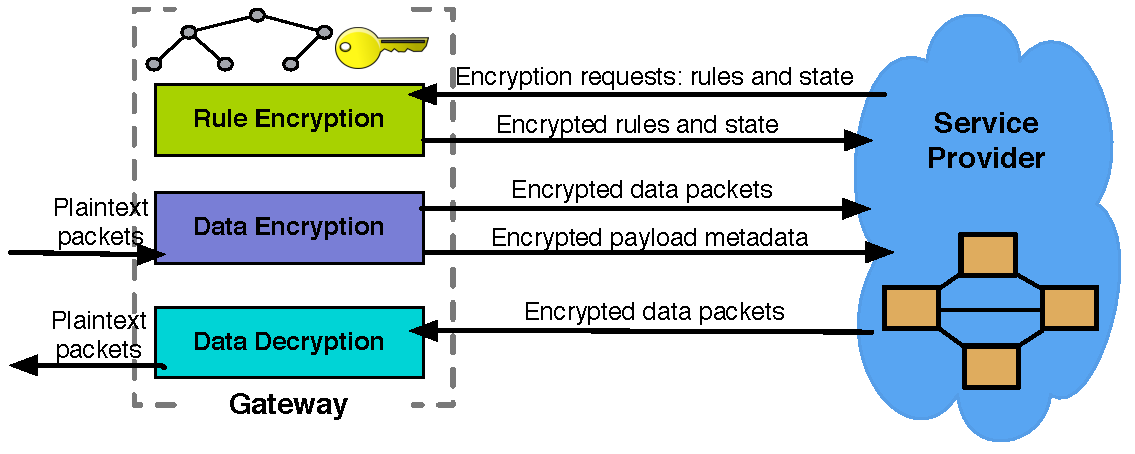
\includegraphics[width=3.25in]{fig/gateway2cloud}
  \caption[]{\label{fig:gatewaymeta} Communication between the cloud and gateway services: rule encryption, data encryption, and data decryption.} 
\end{figure}


%\eat{
%\begin{figure}[t]
%  \centering
%  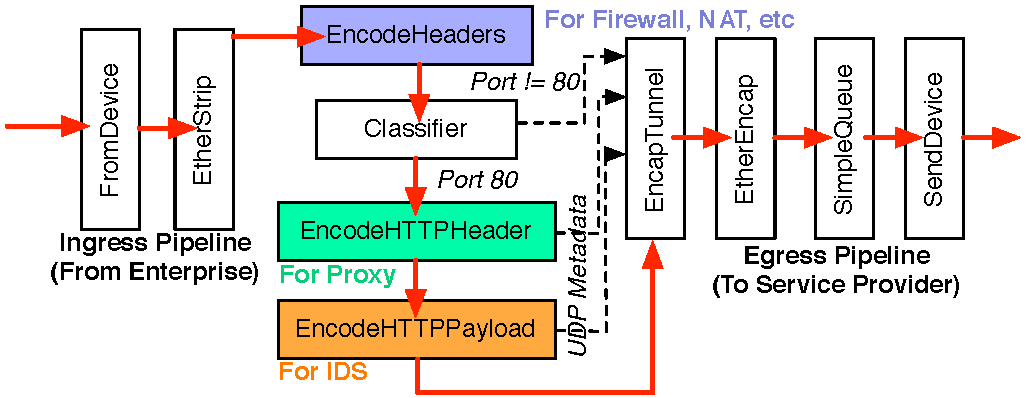
\includegraphics[width=3.25in]{fig/gatewaydiag}
%  \caption[]{\label{fig:gateway} Data encryption (enterprise to cloud) click module.}
%\end{figure}
%}




The gateway serves two purposes. First, it redirects traffic to/from the cloud for middlebox processing. Second, it provides the cloud with encryptions of rulesets.
Every gateway is configured statically to tunnel traffic to a fixed IP address at a single service provider point of presence.
A gateway can be logically thought of as three services: the rule encryption service, the pipeline from the enterprise to the cloud (Data encryption), and the pipeline from the cloud to the enterprise (Data decryption). 
All three services share access to the PrefixMatch state and the private key $k$.
Figure~\ref{fig:gatewaymeta} illustrates  these three services and the data they send to and from the cloud provider.

We design the gateway with two goals in mind: 

\noindent{\bf Format-compatibility}: in converting plaintext traffic to encrypted traffic, the encrypted data should be structured in such a way that the traffic {\it appears as normal IPv6 traffic} to middleboxes performing the processing. Format-compatibility allows us to leave fast-path operations unmodified not only in middlebox software, but also in hardware components like NICs and switches; this results in good performance at the cloud.

\noindent{\bf Scalability and Low Complexity}: the gateway should perform only inexpensive per-packet operations and should be parallelizable. The gateway should not require configuration other than to generate a key and establish a session with the cloud provider. If the gateway were as expensive and complex as the middleboxes, there would be no cost or management benefits from outsourcing. 

%We now discuss how the gateway performs encryption and decryption (\S\ref{sec:dataenc}) and how rules are encrypted (\S\ref{sec:rulenc}) with these design goals in mind.

\subsection{Data Encryption and Decryption}
\label{sec:dataenc}

As shown in Table~\ref{tbl:mbreqs}, we categorize middleboxes as Header middleboxes, which operate only on IP and transport headers; DPI middleboxes, which operate on arbitrary fields in a connection bytestream; and HTTP middleboxes, which operate on values in HTTP headers (these are a subclass of DPI middleboxes). We discuss how each category of data is encrypted/decrypted in order to meet middlebox requirements as follows.

\subsubsection{IP and Transport Headers}
IP and Transport Headers are encrypted field by field (\eg{}, a source address in an input packet results in an encrypted source address field in the output packet) with PrefixMatch.
We use PrefixMatch for these fields because many middleboxes perform analysis over prefixes and ranges of values -- e.g., a firewall may block all connections from a restricted IP prefix.


To encrypt a value with PrefixMatch's EncryptValue, the gateway seeds the encryption with  $\seed = \prf_k(SIP,\ SP,\ DIP,\ DP,\ P)$, a function of both the key and connection information using the notation in Table~\ref{tbl:mbreqs}. Note that in the system setup with two gateways, the gateways generate the same encryption because they share $k$.  


When encrypting IP addresses,  two different IP addresses must not map to the same encryption because this breaks the NAT. To avoid this problem, encrypted IP addresses in \sys must be IPv6 because the probability that two IP addresses get assigned to the same encryption is negligibly low. The reason is that each encrypted prefix contains a large number of possible IP addresses. Suppose we have $n$ distinct firewall rules, $m$ flows and a $\len$-bit space, the probability of a collision is approximately: 

\begin{equation}
1 - e^\frac{-m^2 (2n+1)}{2^{\len+1}}
\end{equation}
% for n firewall rules, there are at most 2n +1 intervals


Therefore, if $\len=128$ (which is the case when we use IPv6), the probability is negligible in a normal setting. 

When encrypting ports, it is possible to get collisions since the port field is only 16-bit. However, this will not break the NAT's functionality as long as the IP address does not collide, because NATs (and other middleboxes that require injectivity) considers both IP addresses and ports. For example, if we have two flows with source IP and source ports of $(SIP, SP_1)$ and $(SIP, SP_2)$ with $SP_1 \neq SP_2$, the encryption of SIP will be different in the two flows because the encryption is seeded in the 5-tuple of a connection. As we discuss in Appendix~\ref{sec:appendix:middleboxes}, the NAT table can be larger for \sys, but the factor is small in practice.




\mypara{Decryption}
PrefixMatch is not reversible. To enable packet decryption, we store the AES-encrypted values for the header fields in the IPv6 options header. 
When the gateway receives a packet to decrypt, if the values haven't been rewritten by the middlebox (\eg, NAT),
it decrypts the values from the options header and restores them. 
% to the IP or transport header.

\mypara{Format-compatibility} 
Our modifications to the IP and transport headers place the encrypted prefix match data back in to the same fields as the unencrypted data was originally stored; because comparisons between rules and encrypted data rely on $\leq$ $\geq$, just as unencrypted data, this means that operations performing comparisons on IP and transport headers {\it remain entirely unchanged at the middlebox.}
This ensures backwards-compatibility with existing software {\it and hardware} fast-path operations.
Because per-packet operations are tightly optimized in production middleboxes, this compatibility ensures good performance at the cloud despite our changes.

An additional challenge for format compatibility is where to place the decryptable AES data; one option would be to define our own packet format, but this could potentially lead to incompatibilities with existing implementations. By placing it in the IPv6 options header, middleboxes can be configured to ignore this data.\footnote{It is a common misconception that middleboxes are incompatible with IP options. Commercial middleboxes are usually aware of IP options but many administrators {\it configure} the devices to filter or drop packets with certain kinds of options enabled.}


\subsubsection{Payload Data} 
The connection bytestream is encrypted with KeywordMatch. Unlike PrefixMatch, the data in all flows is encrypted with the same key $k$. The reason is that KeywordMatch is randomized and it does not leak equality patterns across flows.

This allows \sys to support DPI middleboxes, such as intrusion detection or exfiltration prevention.
These devices must detect whether or not there exists an exact match for an encrypted rule string {\it anywhere} in the connection bytestream.
Because this encrypted payload data is over the {\it bytestream}, we need to generate encrypted values which span `between' packet payloads. 
Searchable Encryption schemes, which we use for encrypted DPI, require that traffic be {\it tokenized} and that a set of fixed length substrings of traffic be encrypted along a sliding window -- e.g., the word malicious might be tokenized into {`malici', `alicio', `liciou', `icious'}.
If the term `malicious' is divided across two packets, we may not be able to tokenize it properly unless we reconstruct the TCP bytestream at the gateway. Hence, if DPI is enabled at the cloud, we do exactly this.

\todo{not clear extension channel}
After reconstructing and encrypting the TCP bytestream, the gateway transmits the encrypted bytestream over 
an `extension', secondary channel that only those middleboxes which perform DPI operations inspect. 
This channel is not routed to other middleboxes. We implement this channel as a persistent TCP connection 
between the gateway and middleboxes. The bytestream in transmission is associated with its flow identifier, 
so that the DPI middleboxes can distinguish between bytestreams in different flows.
DPI middleboxes handle both the packets received from the extension channel as well as the primary channel containing the data packets. 
Hence, if an intrusion prevention system finds a signature in the extension channel, it can sever or reset connectivity for the primary channel.

\noindent{\bf Decryption.} The payload data is encrypted with AES and placed back into the packet payload -- like PrefixMatch, KeywordMatch is not reversible and we require this data for decryption at the gateway.
Because the extension channel is not necessary for decryption, it is not transmitted back to the gateway.

\noindent{\bf Format-compatibility.} To middleboxes which only inspect/modify packet headers, encrypting payloads has no impact. 
By placing the encrypted bytestreams in the extension channel, the extra traffic can be routed past and ignored by middleboxes which do not need this data. % hence it will not interfere with normal processing. 

DPI middleboxes which do inspect payloads must be modified to inspect the extension channel alongside the primary channel, as described in~\cite{blindbox}; DPI devices are typically implemented in software and and these modifications are both straightforward and introduce limited overhead (as we will see in \S\ref{sec:eval}). 

\subsubsection{HTTP Headers} 

HTTP Headers are a special case of payload data. Middleboxes such as web proxies do not read arbitrary values from packet payloads: the only values they read are the HTTP headers. They can be categorized as DPI middleboxes since they need to examine the TCP bytesteam. However, due to the limitation of full DPI support, we treat these values specially compared to other payload data: we encrypt the entire (untokenized) HTTP URI using a deterministic form of KeywordMatch.

Normal KeywordMatch permits comparison between encrypted values and rules, but not between one value and another value; deterministic KeywordMatch permits two values to be compared as well.
Although this is a weaker security guarantee relative to KeywordMatch, it is necessary to support web caching which requires comparisons between different URIs.
The cache hence learns the frequency of different URIs, but cannot immediately learn the URI values.
 This is the only field which we encrypt in the weaker setting.
We place this encrypted value in the extension channel; hence our HTTP encryption has the same format-compatibility properties as other DPI devices.

Like other DPI tasks, this requires parsing the entire TCP bytestream. However, in some circumstances we can extract and store the HTTP headers statelessly; so long as HTTP pipelining is disabled and packet MTUs are standard-sized (>1KB), the required fields will always appear contiguously within a single packet. Given that SPDY uses persistent connections and pipelined requests, this stateless approach does not apply to SPDY.
%Hence, if DPI is disabled we can avoid reconstructing the TCP bytestream at the middlebox.
%When DPI is enabled, the gateway scans through every byte of data in the connection already;  extracting these headers allows the middlebox to avoid re-doing work which has already been done at the gateway.

\noindent{\bf Decryption.} The packet is decrypted as normal using the data stored in the payload; IP options are removed.


%\eat{
%JS: I vote to cut this. Here's why -- we are going to be basically hosed when it comes to bandwidth, whether or not we have this. And adding this in adds a huge amount of complexity to the gateway! So way sacrifice our primary goal (cheap, less complex) to only partially fix another problem??
%\subsubsection{Optimizing Decryption}
%To reduce bandwidth usage, the gateway temporarily caches the packets destined to the service provider indexed by their hashes for a short time. If the middleboxes on the cloud do not change the packet content, instead of sending the whole packet back, the service provider sends a control packet containing the hash of the original packet. The gateway then retrieves the local packet by looking up the hash in the cache.
%}

\subsection{Rule Encryption}
\label{sec:rulenc}

Given a ruleset for a middlebox type, the gateway encrypts this ruleset with either KeywordMatch or PrefixMatch, depending on the encryption scheme used by that middlebox as in Table~\ref{tbl:mbreqs}. For example, firewall rules are encrypted using PrefixMatch. As a result of encryption, some rulesets expand and we evaluate in \S\ref{sec:eval} by how much. For example, a firewall rule containing an IP prefix that maps to two encrypted prefixes using PrefixMatch becomes two rules, one for each encrypted prefix.
 


Rules for firewalls and DPI services come from a variety of sources and can have different policies regarding who is or isn't allowed to know the rules. 
For example, exfiltration detection rules may include keywords for company products or unreleased projects which the client may wish to keep secret from the cloud provider. 
On the other hand, many DPI rules are proprietary features of DPI vendors, who may allow the provider to learn the rules, but not the client (gateway).
\sys supports three different models for KeywordMatch rules which allow clients and providers to share rules as they are comfortable: (a) the client knows the rules, and the provider does not; (b) the provider knows the rule, and the client does not; or (c) both parties know the rules.
PrefixMatch rules only supports (a) and (c) -- the gateway {\it must} know the rules to perform encryption properly.

If the client is permitted to know the rules, they encrypt them -- either generating a KeywordMatch, AES, or PrefixMatch rule -- and send them to the cloud provider. If the cloud provider is permitted to know the rules as well, the client will send these encrypted rules annotated with the plaintext; if the cloud provider is not allowed, the client sends only the encrypted rules in random order.

If the client (gateway) is not permitted to know the rules, we must somehow allow the cloud provider to learn the encryption of each rule with the client's key. This is achieved using a classical combination of Yao's garbled circuits~\cite{Yao86} with oblivious transfer~\cite{Naor-Pinkas}, as originally applied by BlindBox~\cite{blindbox}.
As in BlindBox, this exchange only succeeds if the rules are signed by a trusted third party (such as McAffee, Symantec, or EmergingThreats) -- the cloud provider should not be able to generate their own rules without such a signature as it would allow the cloud provider to read arbitrary data from the clients' traffic.
Unlike BlindBox, this rule exchange occurs exactly once -- when the gateway initializes the rule. 
After this setup, all connections from the enterprise are encrypted with the same key at the gateway.
%This is important because for a typical industry ruleset, a garbled circuit + oblivious transfer exchange takes 97 seconds~\cite{blindbox}; with BlindBox this exchange must be performed for every connection and thus is prohibitive for practicality.
%For \sys, on the otherhand, this amounts to a relatively cheap one-time setup cost.

%\eat{
%\subsection{Discussion}
%\label{sec:gwimpl}
%We built our gateway as described above using BESS~\cite{bess} on an off-the-shelf 16-core server with 2.6GHz Xeon E5-2650 cores and 128GB RAM; the network hardware is a single 10GbE Intel 82599 compatible network card. 
%We discuss a few systems properties of our gateway as follows before discussing middlebox implementations in \S\ref{sec:mbimpl}.
%
%\eat{
%Our gateway datapath implementation has 3 major components: Header Rewrite, Stream Reconstruction, and Packet Cache. We primarily introduce the dataflow from the client to the gateway below:
%
%\noindent\textbf{Header Rewrite.} At this stage, the gateway rewrites the header fields in the packets using the PrefixMatch scheme using in algorithm in Section \ref{sec:dataenc}. It consists of multiple Click elements: ProtocolTranslator46 that translates an IPv4 packet to an IPv6 packet, AppendIP6Option that populates DET-encrypted header fields into the IPv6 options, HeaderEncrypt that performs the encryption, and SetTCPChecksum that sets the checksum.
%
%\noindent\textbf{Stream Reconstruction.} This component acts as a TCP transparent proxy by terminating incoming TCP connections from clients. It encrypts the reconstructed bytestreams using the stream cipher, and relays them in new connections. Note that the IP options are preserved during this phase. It also pushes bytestreams into the secondary channel, where middleboxes can perform DPI operations. Meanwhile, it extracts HTTP headers from the stream and puts the deterministically encrypted HTTP header fields into the IP options.
%
%\noindent\textbf{Packet Cache.} The dataflow from the service provider back to the gateway is relatively simple. The Packet Cache restores the packets, the Stream Reconstruction component decrypts the streams into plaintext, then the Header Rewrite component decrypts the header fields and performs 6to4 translation (if the client uses IPv4).
%
%Having discussed the design and implementation of the gateway, we now revisit a few of its system properties before moving on to the design and implementation of the middleboxes in \S\ref{sec:mbimpl}.
%}
%
%\noindent\textbf{Scalability.}
%Encryption and decryption are entirely parallel: they require no synchronization or communication between threads. We show in \S\ref{sec:eval} that we achieve almost linear improvements from adding additional processing cores.
%However, per-packet operations rely only on relatively inexpensive techniques; the most expensive operation performed is AES encryption with is supported in hardware through the AES-NI instructions. 
%Consequently, the gateway can support 10Gbps of traffic with only 8 cores enabled.
%
%\noindent\textbf{Complexity.}
%An administrator only supplies the gateway with the IP address of the cloud and the secret key $k$.
%The administrator places the gateway at the border of their enterprise network to the Internet.
%The administrator supplies any rules/policies to the cloud provider and the gateway is then configured by the cloud provider.
%
%\noindent\textbf{Fault Tolerance.}
%When DPI is disabled, the gateway keeps no per-connection state. Hence, a cold standby can take over correctly for the gateway so long as it has the `static' state of the PrefixMatch tree, key $k$, and IP address of SP.
%When DPI is enabled, the gateway maintains the last few packets from each connection (window-length) to perform tokenization; under these conditions the gateway can use standard techniques for backup including an active standby~\cite{colo}.
%}





% We now describe the procedure for AddRange which adds an interval (deleting an interval is similar). These procedures modify the state at the gateway. To add a range [$s$, $e$], the gateway inserts these values in the tree. If the tree needs to be rebalanced, for each endpoint that changed location in the tree, the gateway records the old and new encrypted value based on the tree in a list $L$. Note that  the number of endpoints that change encryption is $O(\log n)$ amortized worst-case. The gateway then computes the encryption of $s$ and $e$ based on their location in the tree. It sends to SP $\enc(s)$ and $\enc(e)$ along with $L$. 

%Besides the interval added or deleted, a small number
%of other intervals may be moved -- at worst, $O(\log n)$. 
%For these, the algorithm returns the old and new encryption of the interval. 

%
%\begin{framed}
%\begin{algorithmic}[1]
%
%\Procedure{AddRange}{$[s, e]$}
%  \State Insert $s$ and $e$ into the scapegoat tree. If $s=e$, insert the value only once.
%  %	
%  \State Initialize $L$ to be the empty list.
%  \If{tree needs to be rebalanced}
%  	\State Record which nodes change position in the tree during rebalancing, together with 
%	their old and new encryptions. Namely, record	\[L = \{ \en_1 \leftarrow \en^*_1, \dots, \en_m \rightarrow \en^*_m\},\] where $m$ is the number of nodes who changed position in the tree, and $\en_i$ and $\en^*_i$ are the old and new encryption of the $i$-th node that changed position. 
%  \EndIf
%  \State Compute  $\enc(s)$ and $\enc(e)$, the encryptions of $s$ and $e$, as in EncryptRanges.
%   \State \Return{$[\enc(s), \enc(e)], L$}
%\EndProcedure
%
%\end{algorithmic}
%\end{framed}

%  \State Determing the smallest and the largest encryption in the values $[\enc(s), \enc(e)]$ and $L$, and call this $\dirtyrange$.



\mypara{Rule Updates}
\label{sec:updates}
%
Rule updates need to be treated carefully for PrefixMatch.
Adding a new prefix/range or removing an existing range can affect the encryption of an existing prefix. The reason is that the new prefix can overlap with an existing one. In the worst case, the encryption of all the rules needs to be updated. 

The fact that the encryption of old rules changes poses two challenges.
The first challenge is the correctness of middlebox state. Consider a NAT with a translation table containing ports and IP addresses for active connections. The encryption of an IP address with EncryptValue depends on the list of prefixes so an IP address might be encrypted differently after the rule update, becoming inconsistent with the NAT table.
 Thus, the NAT state must also be updated.
The second challenge is a race condition: if the middlebox adopts a new ruleset while packets encrypted under the old ruleset  are still flowing, these packets can be misclassified.
%The same problem occurs if packets encrypted under the new ruleset arrive before the new ruleset was .


\todo{ explain better buffering and upper bound if it suffices not to mix new and old packets}
To avoid these problems, the gateway and the cloud provider do the following. 
The gateway first runs EncryptPrefixes for the new set of prefixes and creates a new set of encrypted prefixes and a new interval map. 
Then, the gateway announces to the cloud provider the pending update, and the middleboxes ship their current state to the gateway. The gateway updates this state by producing new encryptions and sends the new state back to the middleboxes. During all this time, the gateway continued to encrypt traffic based on the old prefixes and the middleboxes processed it based on the old rules.
Once all middleboxes have the new state, the gateway sends a signal to the cloud provider that it is about to `swap in' the new data. 
The cloud provider buffers traffic for a few hundred milliseconds after this signal to allow all old traffic to complete processing at the cloud; it signals to all middleboxes to `swap in' the new rules and state; and finally it starts processing new traffic.
Note that all changes to middleboxes are in the {\it control plane} of the middlebox, and require no modifications to the algorithms and operations performed in per-packet processing. 

\todo{fix para below:}
The cloud provider updating middlebox rules will have to write rules appropriately to account for the fact that a 
single prefix maps to multiple intervals. For example, suppose there is a middlebox that counts the number 
of connections to a prefix $P$. $P$ maps to a single interval $I$. After updating, a new prefix is added 
which  partially overlaps with $P$. Hence $I$ becomes $I_1$ and $I_2$. The cloud provider should update 
rules appropriately. If the logic before the update is `\texttt{if $v$ in $I$ then counter++}',
it should become `\texttt{if $v$ in $I_1$ or $v$ in $I_2$ then counter++}'.





\todo{webproxy is it on top of squid or if not, why did not compare to without enc}

\todo{clarify that is the baseline}

\todo{explain regexp protocol expansion}





\section{Middleboxes: Design \& Implementation}
\label{sec:mbs}

In Table~\ref{tbl:mbreqs}, we introduced the set of middleboxes typically supported by outsourcing approaches and divided them in to Header, HTTP, and DPI middleboxes. 
We now revisit these middleboxes individually and discuss how they operate over the encrypted data.

\eat{
\begin{figure}[t]
  \centering
  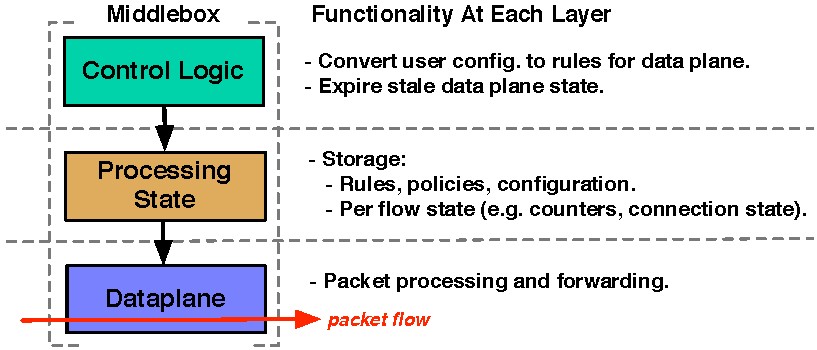
\includegraphics[width=3in]{fig/mbarch}
  \caption[]{\label{fig:mbarch} Typical middlebox software components. For most middleboxes, packet processing operations in the dataplane remain unmodified by \sys. \justine{Cut? Unnecessary?}}
\end{figure}
}

\subsection{Header Middleboxes}
Middleboxes which operate on IP and transport headers only include firewalls, NATs, and L4 load balancers.
Firewalls are read-only, but NATs and L4 load balancers may rewrite IP addresses or port values. 
For header middleboxes, per-packet operations remain unchanged for both read and write operations.

For read operations, the firewall receives a set of encrypted rules from the gateway and compares them directly against the encrypted packets just as normal traffic. Because RangeMatch supports $\leq$ and $\geq$, the firewall may use any of the standard classification algorithms~\cite{packet_classif}.

For write operations, the middleboxes assign values from an address pool; it receives these encrypted pool values from the gateway during the rule generation phase.
These encrypted rules are marked with a special suffix reserved for rewritten values.
When the gateway receives a packet with such a rewritten value, it restores the plaintext value from the pool rather than decrypting the value from the options header.

\subsection{DPI Middleboxes}
We modify middleboxes which perform DPI operations as described by BlindBox~\cite{blindbox}; unlike header middleboxes these devices must be rewritten in per-packet behavior to support encrypted traffic.
The middleboxes search through the encrypted extension channel -- not the packet payloads themselves -- and block the connection if a blacklisted term is observed in the extension.

\subsection{HTTP Middleboxes}
Parental filters and L7 Load Balancers read the HTTP URI from the options header. 
If the parental filter observes a blacklisted URI, it drops the connection.
The L7 load balancer uses the URI to rewrite the IP header, and operates exactly like a NAT or L4 LB, except that it uses the URI to select which destination address to assign new connections.

The proxy required the most modification of any middlebox \sys supports; nonetheless, our proxy achieves good performance as we will discuss in \S\ref{sec:eval}.
The proxy  caches HTTP static content (e.g., images) in order to improve client-side performance. 
When a client opens a new HTTP connection, a typical proxy will capture the client's SYN packet and open a new connection to the client, as if the proxy were the web server. The proxy then opens a second connection in the background to the original web server, as if it were the client. 
When a client sends a request for new content, if the content is in the proxy's cache, the proxy will serve it from there. Otherwise, the proxy will forward this request to the web server and cache the new content. 

The proxy has a map of encrypted file path to encrypted file content. When the proxy receives a packet, the proxy extracts the encrypted URI from the options header and looks it up in the cache {\em as if it were not encrypted}. The use of deterministic encryption enables the proxy to use a fast search data structure/index, such as a hash map, unchanged. We have two cases: there is a hit or a miss. For hit, the proxy assembles a packet header for reverse traffic and attaches to it the encrypted file content from the cache. Even without being able to encrypt IP addresses or ports, the proxy can create the header by reversing the encrypted information in the original header.
For a miss, the proxy forwards the request to the web server. When receiving the response, the proxy caches it to serve future requests.




%!TEX root = mb.tex
\begin{figure}[t]
  \centering
  \begin{tabular}{cc}
  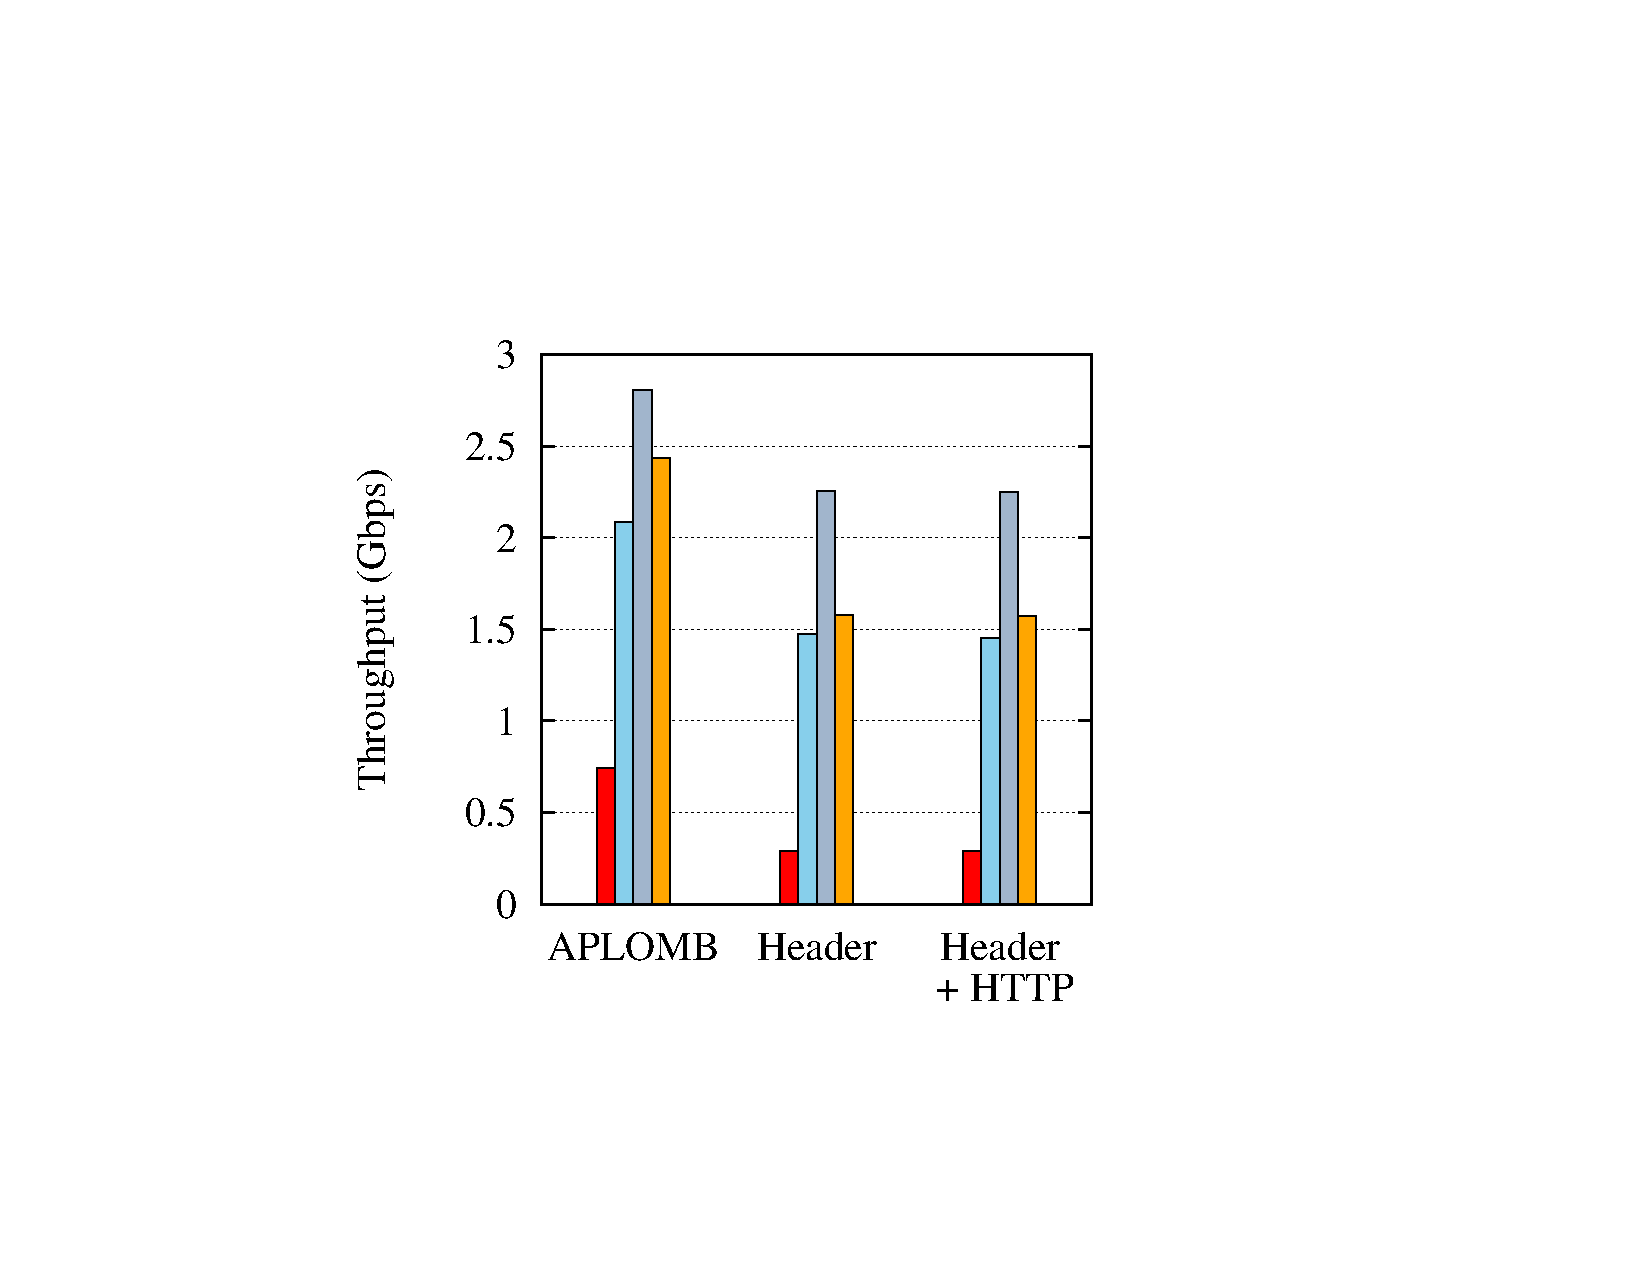
\includegraphics[height=1in]{fig/gatewayxput}&
  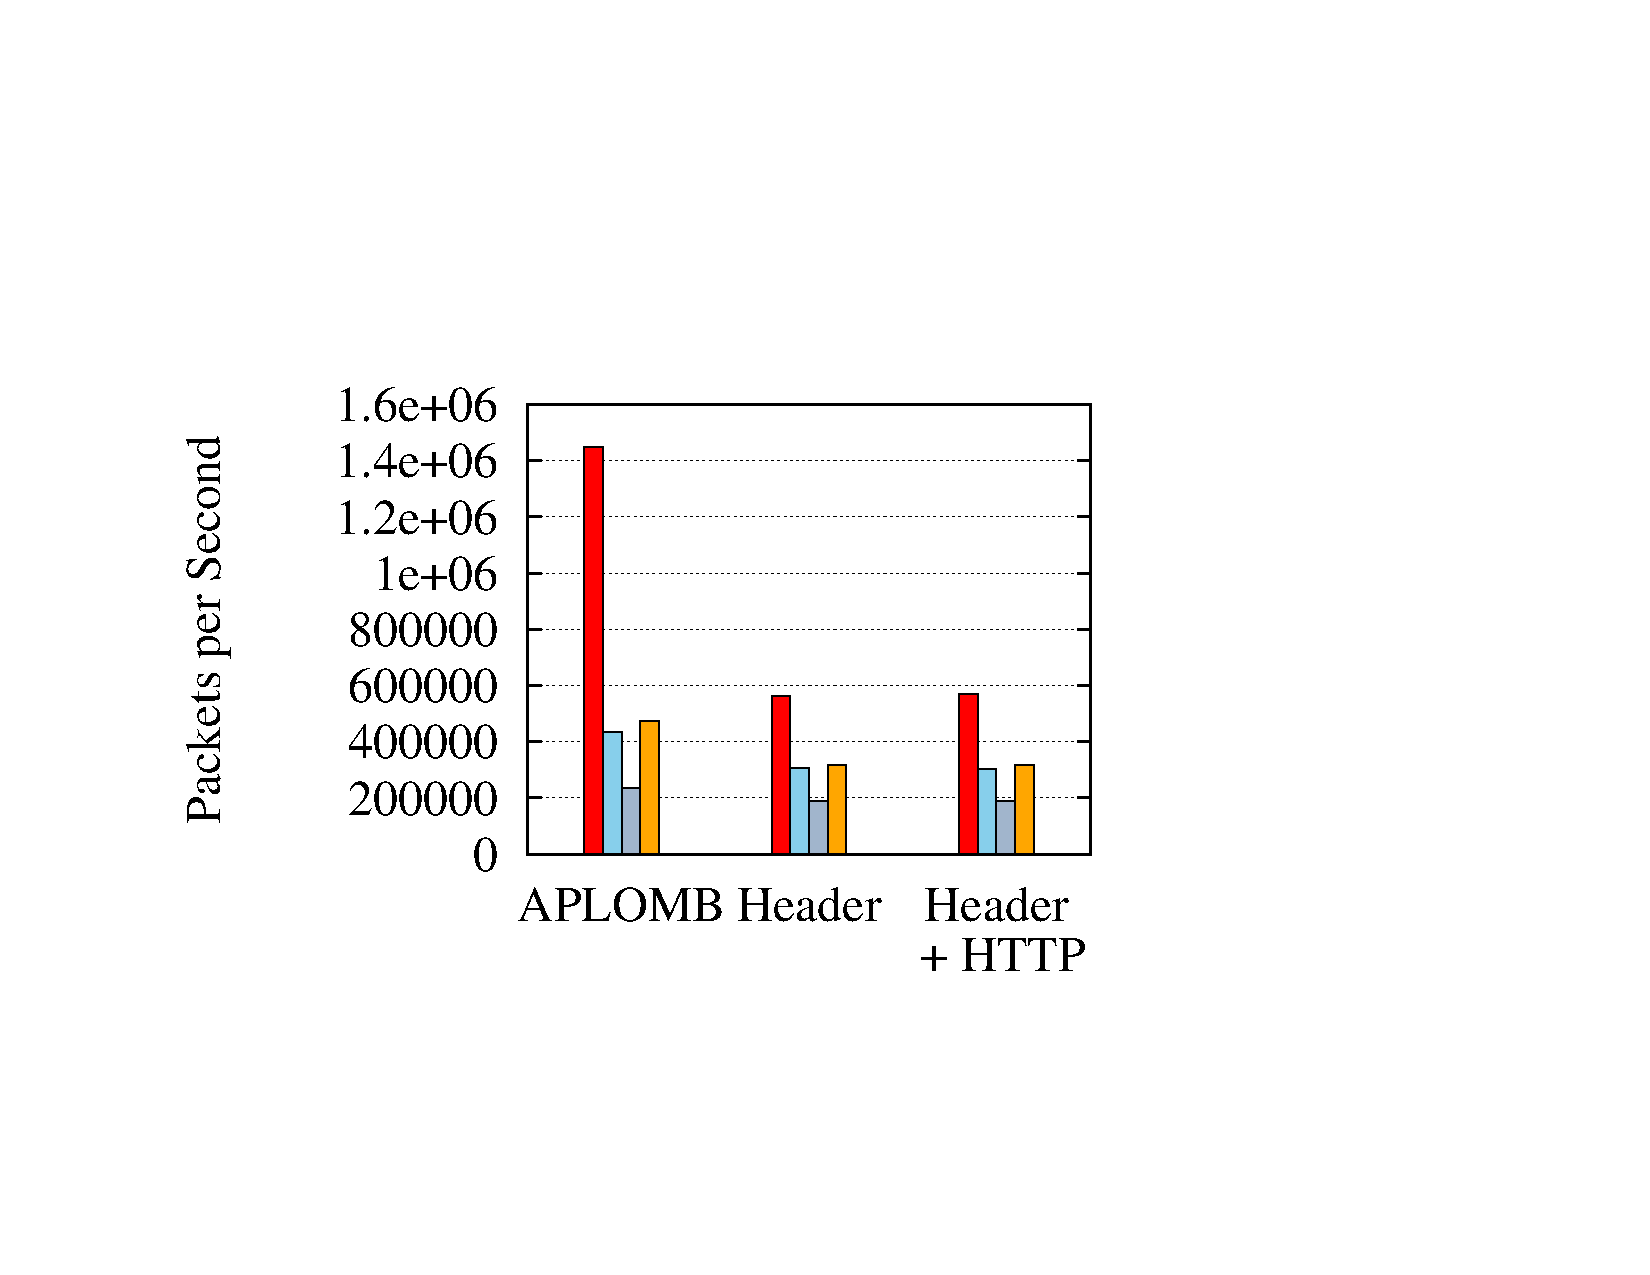
\includegraphics[height=1in]{fig/gateway_pps}\\
  \end{tabular}
  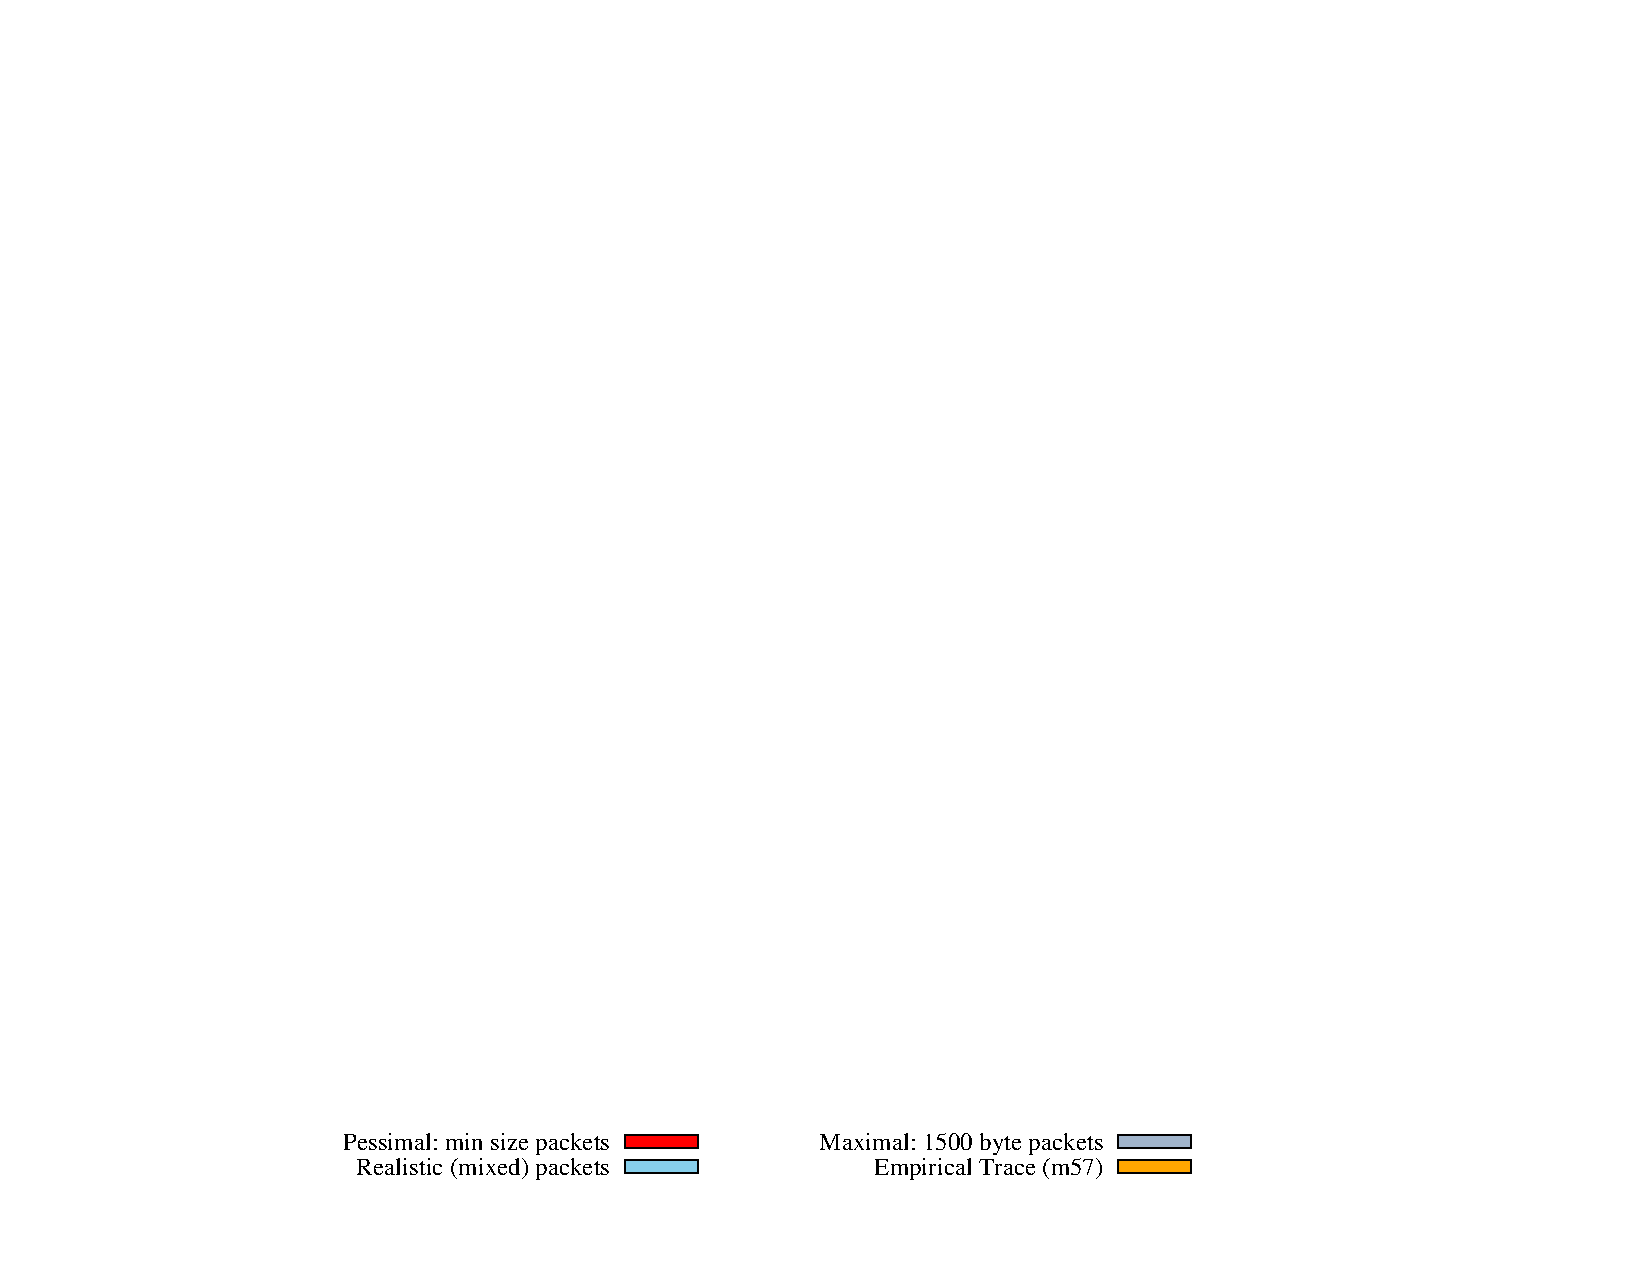
\includegraphics[width=2.75in]{fig/key}
  \caption[]{\label{fig:gwxput} Throughput/Packets per Second on a single core at the stateless gateway.}
\end{figure}

\begin{figure}[t]
  \centering
  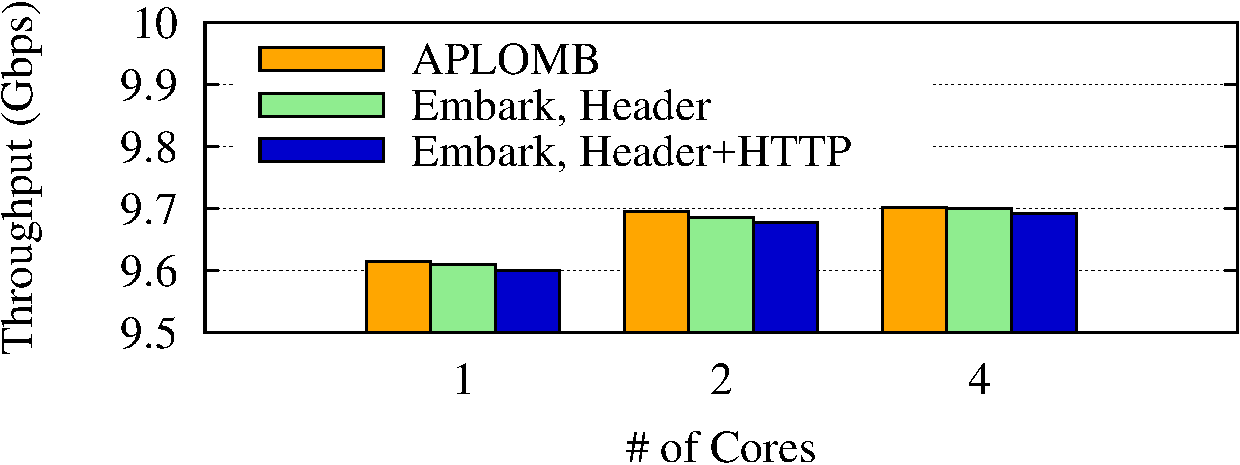
\includegraphics[width=3in]{fig/gateway_scale}
  \caption[]{\label{fig:gwscale} Gateway throughput with increasing parallelism.}
\end{figure}
 
\section{Evaluation} \label{sec:eval}

As we showed in \S\ref{sec:mbs}, \sys supports all middlebox applications in typical outsourcing environments~\cite{aplomb,etsi-nfv}. Hence, from a functionality perspective, \sys answers our original question, ``Is it possible to enable a third party to perform traffic processing for an enterprise, {\em without seeing the enterprise's traffic}?''  strongly in the affirmative.

We now investigate whether \sys is practical from a performance perspective, looking at the overheads due to encryption and redirection. 
We built our gateway using Click~\cite{click} over DPDK~\cite{dpdk} on an off-the-shelf 16-core server with 2.6GHz Xeon E5-2650 cores and 128GB RAM; the network hardware is a single 10GbE Intel 82599 compatible network card. 
We deployed our prototype gateway in our research lab and redirected traffic from a 3-server testbed through the gateway; these three client servers had the same hardware specifications as the server we used as our gateway.
We deployed our middleboxes on Amazon EC2.
For most experiments, we use a synthetic workload generated by the Pktgen~\cite{pktgen}; for experiments where an empirical trace is specified we use the m57 patents trace~\cite{m57} and the ICTF 2010 trace~\cite{ictf}.

%In what follows, we evaluate our performance at the enterprise, including gateway throughput, end-to-end page load times, and bandwidth costs (\S\ref{sec:enterprise}). We then evaluate performance at the cloud, evaluating each middlebox we implemented one by one (\S\ref{sec:evalcloud}).

\subsection{Enterprise Performance}
\label{sec:enterprise}
We first evaluate \sys's overheads at the enterprise. %including the gateway, end-to-end performance, and bandwidth costs from deploying \sys.

\subsubsection{Gateway}

 
\noindent{\it How many servers does a typical enterprise require to outsource traffic to the cloud?}
Figure~\ref{fig:gwxput} shows the gateway throughput when encrypting traffic to send to the cloud, first with normal redirection (as used in APLOMB~\cite{aplomb}), then with \sys's L3/L4-header encryption, and finally with L3/L4-header encryption as well as HTTP/proxy encryption. 
For empirical traffic traces with payload encryption (DPI) disabled, \sys averages 1.5Gbps per core; for full-sized packets it achieves over 2Gbps.
In scalability experiments (Fig.~\ref{fig:gwscale}) with eight cores dedicated to processing, our server could could forward at up to 8Gbps while encrypting for headers and HTTP traffic.
There is little difference between the HTTP overhead and the L3/L4 overhead, as the HTTP encryption only occurs on HTTP requests -- a small fraction of packets. 
With DPI enabled (not shown), throughput dropped to 240Mbps per core, suggesting that an enterprise would need to devote at least 32 cores to the gateway.
%Overall, \sys encryption for the stateless gateway reduces by about 60\% relative to baseline APLOMB encryption in the worst case (the min-sized workload; the reduction for the empirical (m57) workload is 38\%.  

\begin{figure}[t]
  \centering
  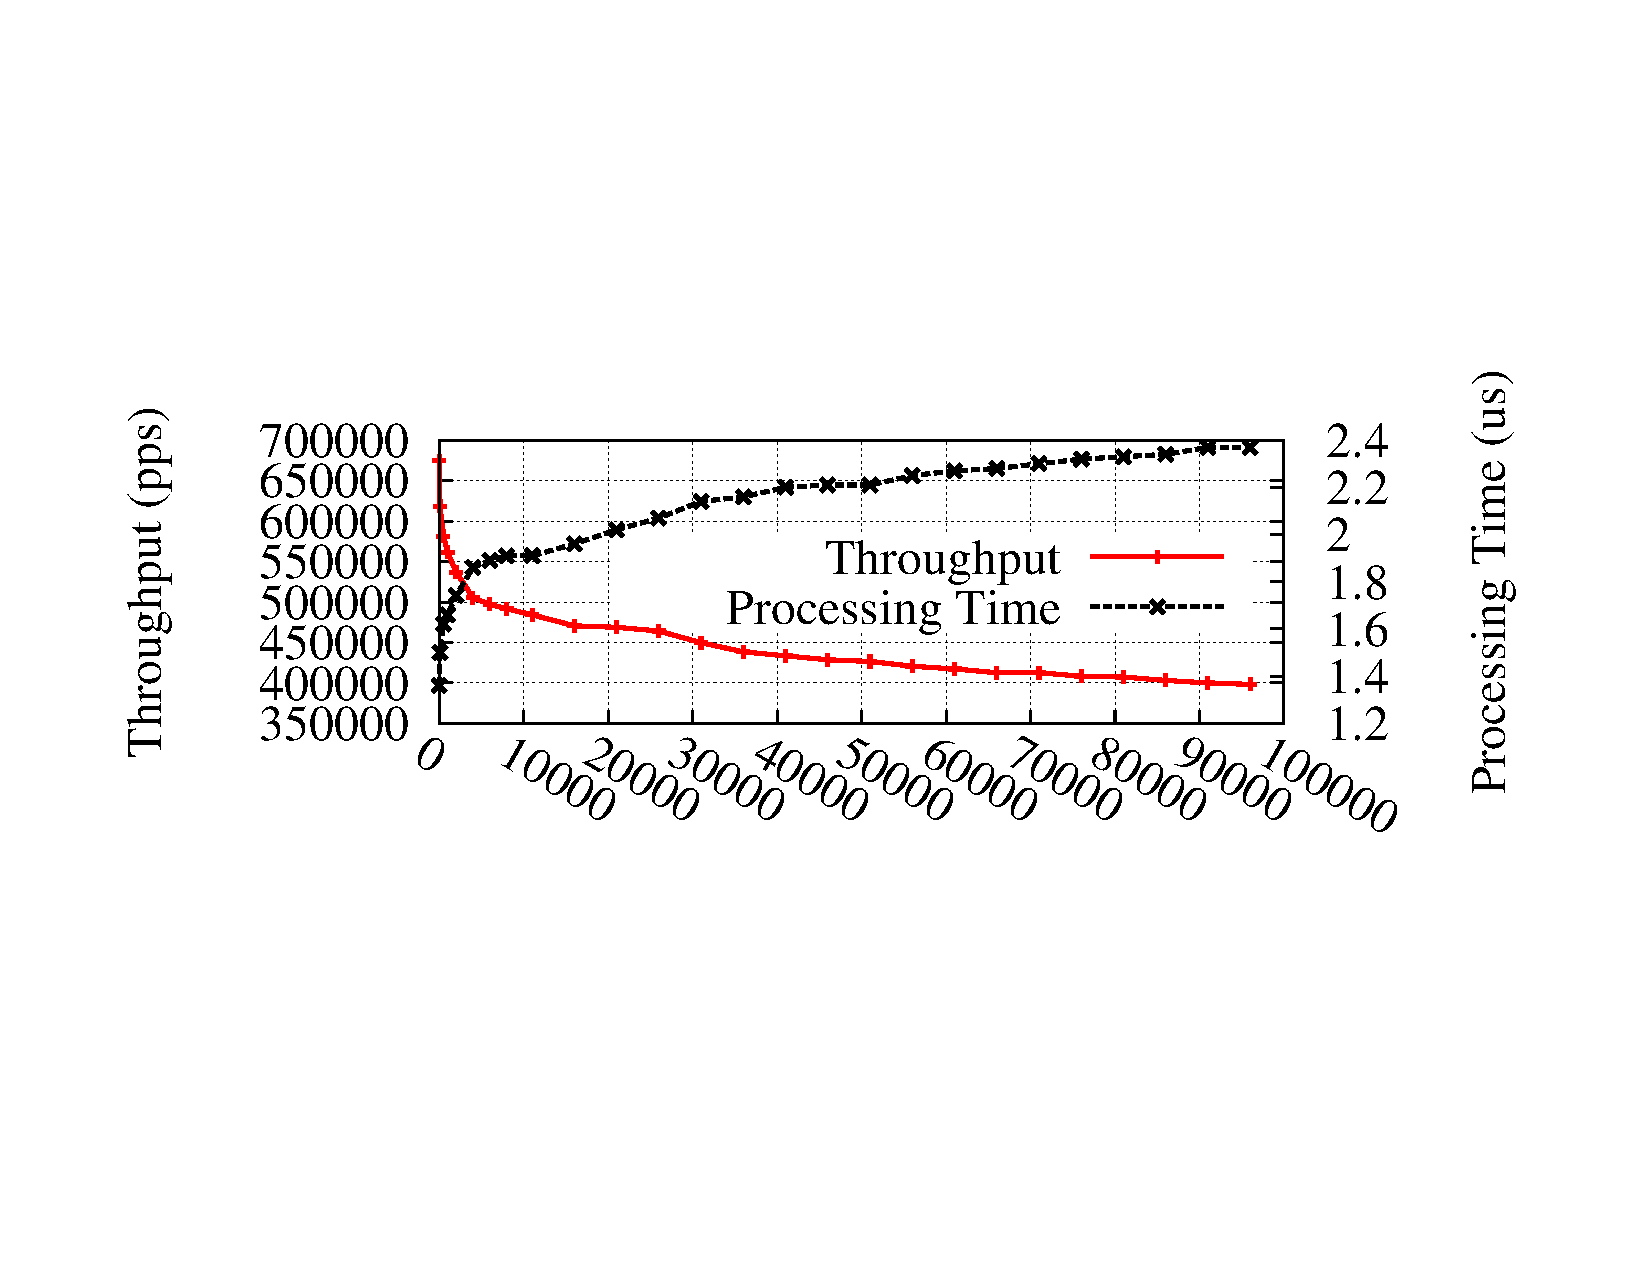
\includegraphics[width=3in]{fig/xputrange}
  \caption[]{\label{fig:xputrange} Throughput as number of rules for range encrypt increases.}
\end{figure}

\noindent{\it How do throughput and latency at the gateway scale with the number of rules for range encryption?} 
In \S\ref{sec:range}, we discussed how our range encryption scheme stores encrypted values in a tree; every packet encryption requires a traversal of this tree.
Hence, as the size of the tree goes larger, we can expect to require more time to process each packet and throughput to decrease.
We measure this effect in Figure~\ref{fig:xputrange}. 
On the $y_1$ axis, we show the aggregate per packet throughput at the gateway as the number of rules from 0 to 100k. The penalty here is logarithmic, which is the expected performance of tree data structures. From 0-10k rules, throughput drops from 670Kpps to 480Kpps; after this point the performance penalty of additional rules tapers off. Adding an additional 90k rules drops throughput to 400Kpps.
On the $y_2$ axis, we measure the processing time per packet, \ie{}, the amount of time for the gateway to encrypt the packet; the processing time follows the same logarithmic trend.

\noindent{\it Is range encryption faster than existing order preserving algorithms?}
RangeMatch is the only encryption scheme that has low latency and the ordering property needed for packet processing.
We compare against BCLO~\cite{boldyreva:ope} and mOPE~\cite{popa:mope} below:

\begin{table}[h]
\vspace{-10pt}
\centering
\small
\begin{tabular}{c|c|c|c}
{\bf Operation}&{\bf BCLO}&{\bf mOPE}&{\bf \sys}\\
\hline
\hline
Encrypt, 10K rules&9333$\mu$s&6640$\mu$s&1.95$\mu$s\\
\hline
Encrypt, 100K rules&9333$\mu$s&8300$\mu$s&3$\mu$s\\
\hline
Decrypt&169$\mu$s&0.128$\mu$s&0.128$\mu$s\\
\hline
\end{tabular}
\vspace{-10pt}
\end{table}

\noindent{\it What is the memory overhead of the stateful range map encryption scheme?}
Storing 10k rules in memory requires 1.6MB, and storing 100k rules in memory requires 28.5MB -- using unoptimized C++ objects.
This state overhead is negligible on any modern server.

\subsubsection{Client Performance}

\begin{figure}
  \hspace{-15pt}
%  \begin{tabular}{cccc}
%  
\includegraphics[height=1in]{fig/cdflabel}
%  &\hspace{-10pt}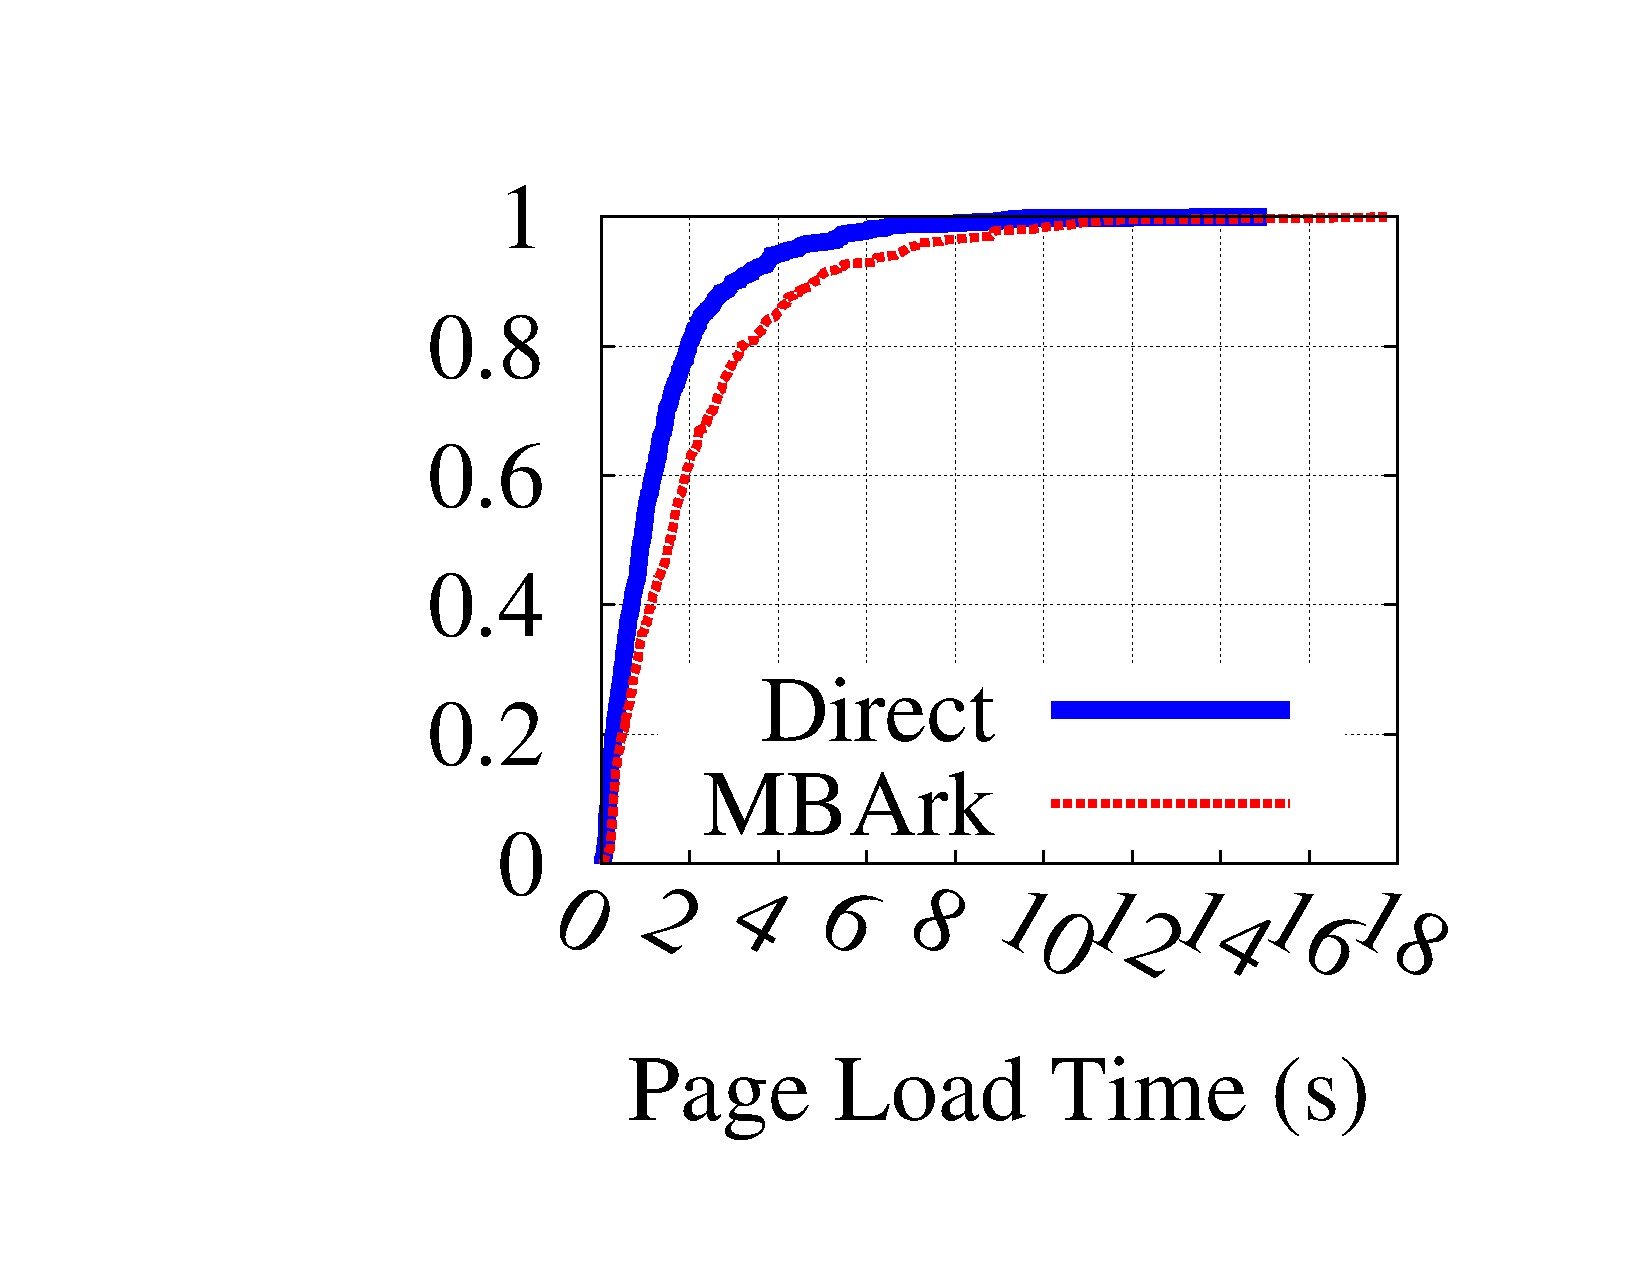
\includegraphics[height=.9in]{fig/e2e_loadtimes}
%  &\hspace{-10pt}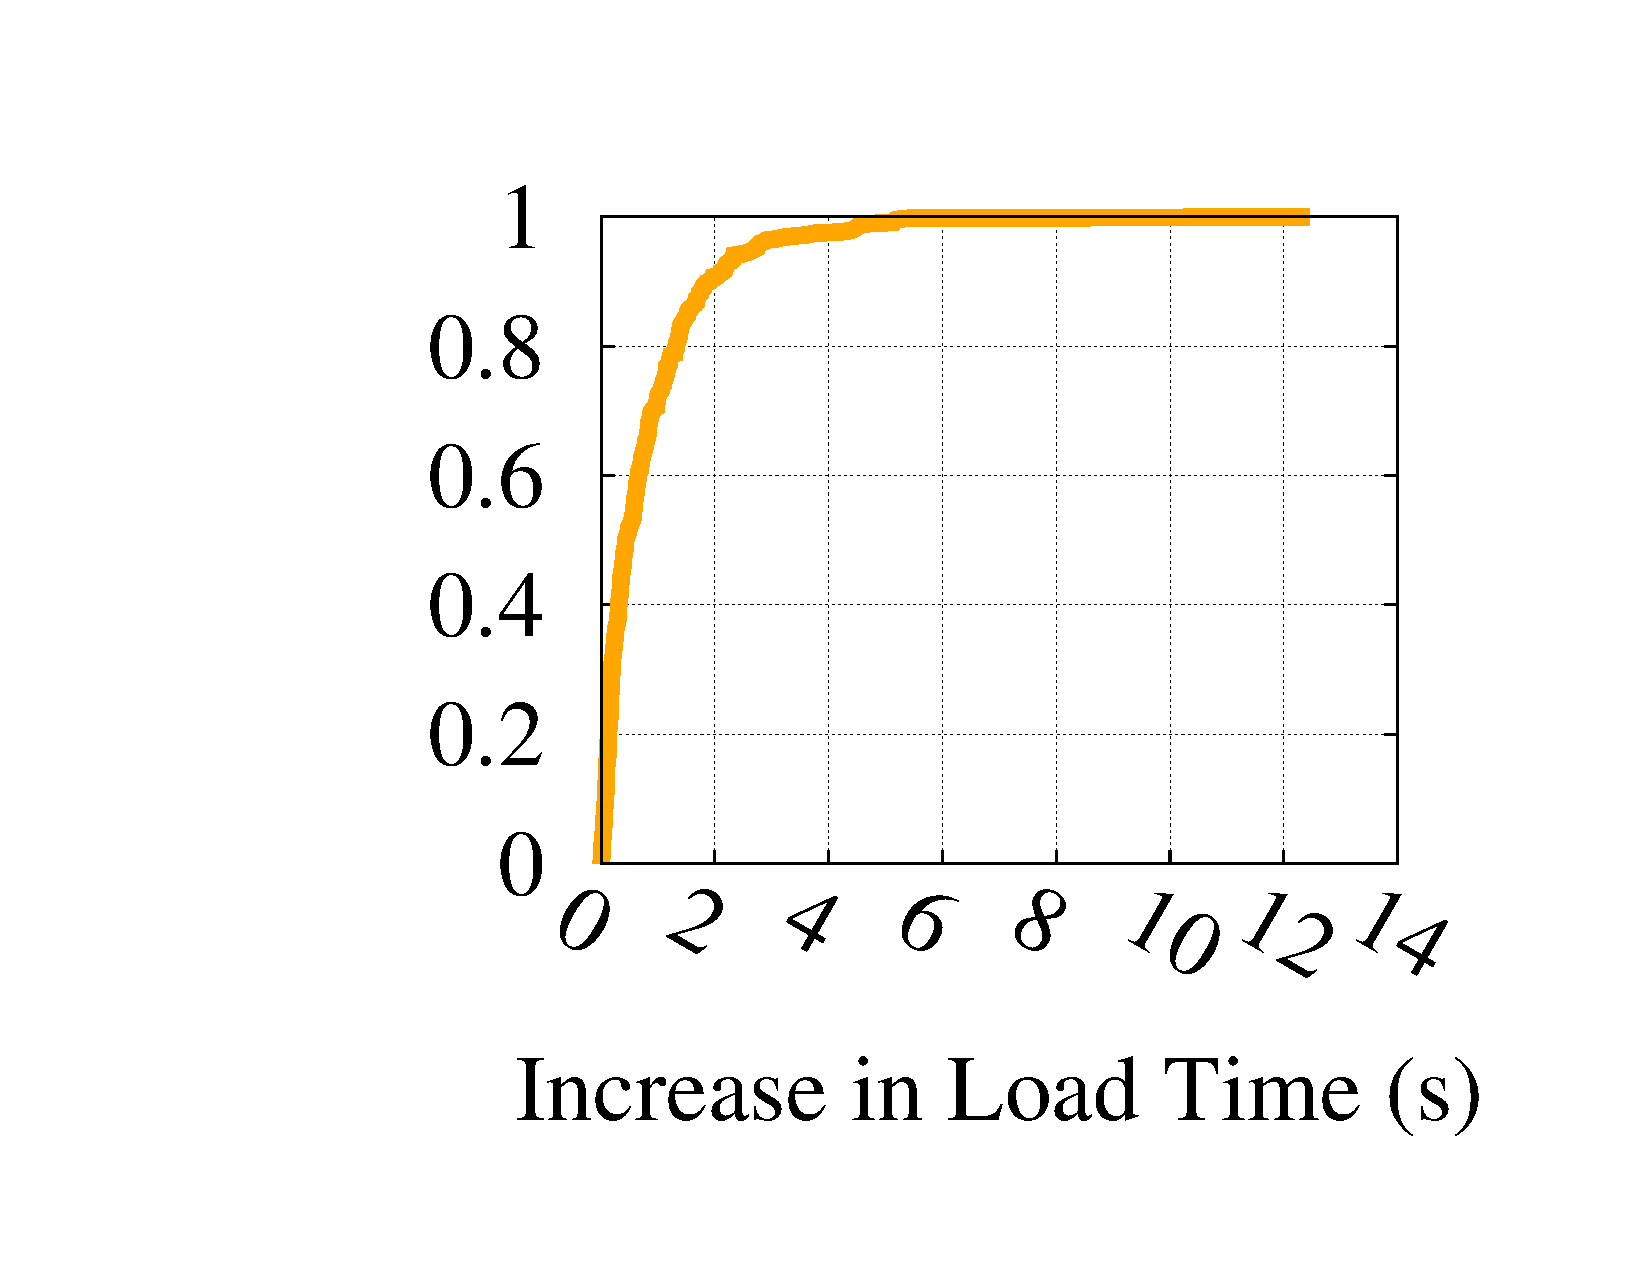
\includegraphics[height=.9in]{fig/e2e_delta_absolute}
%  &\hspace{-10pt}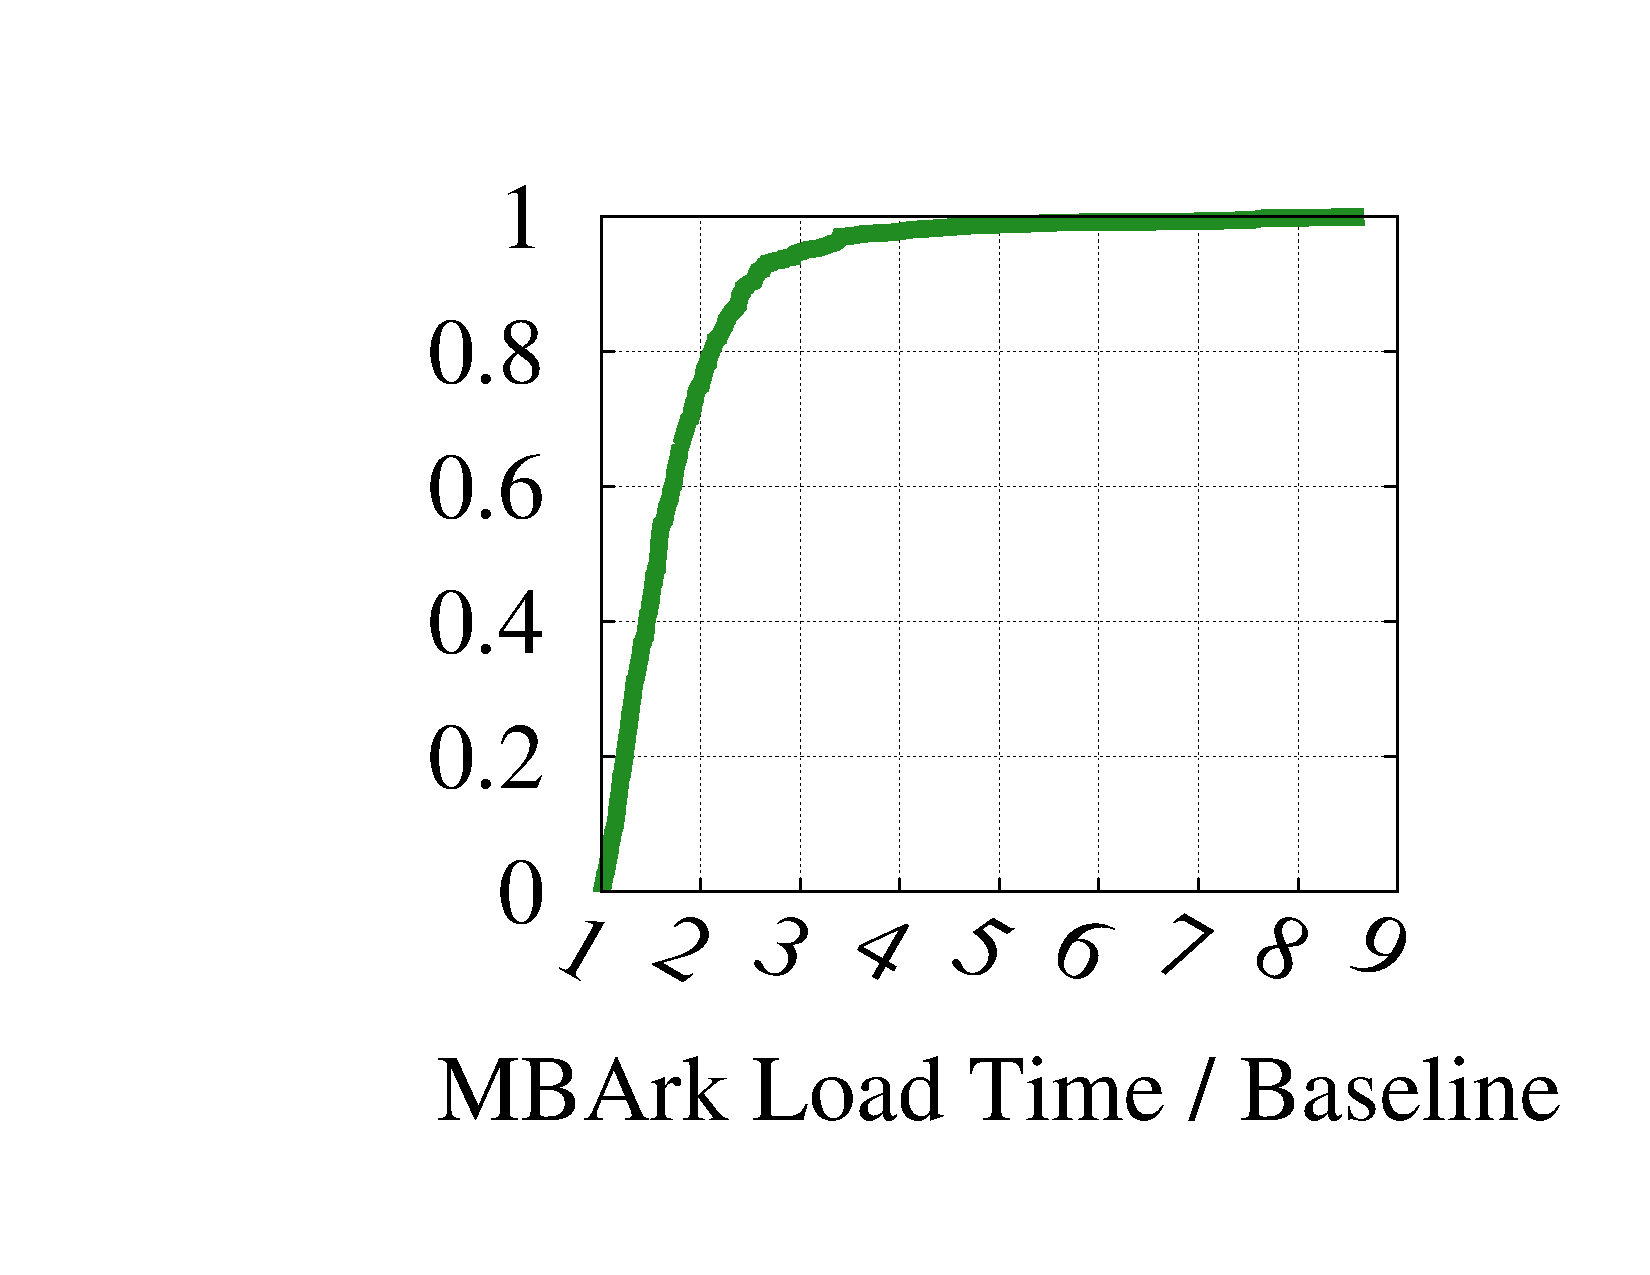
\includegraphics[height=.9in]{fig/e2e_delta_relative}
%  \\
%  &(a)&(b)&(c)\\
%  \end{tabular}
  \centering
  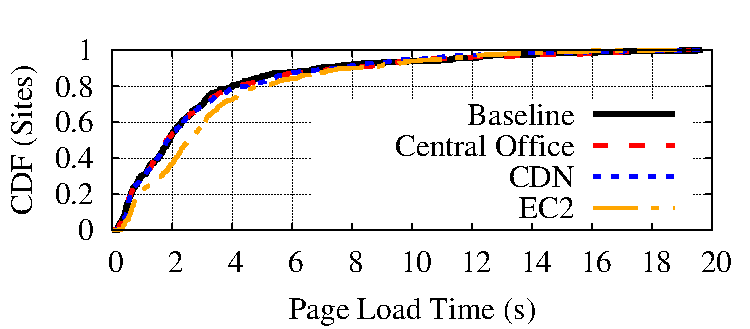
\includegraphics[width=2.7in]{fig/e2e_compare}
  \caption[]{\label{fig:e2eloads} Page load times under different deployments.}
\end{figure}

We use web performance to understand end-to-end user experience of \sys.
Figure~\ref{fig:e2eloads} shows a CDF for the Alexa top-500 sites loaded through our testbed. We compare the baseline (direct download) assuming three different service providers: an ISP hosting services in a Central Office (CO), a Content-Distribution Network EC2, and a traditional cloud provider (EC2). We deployed \sys on EC2 and used this deployment for our experiments, but for the CO and CDN experiments we emulated the deployment with inflated latencies and servers in our testbed. 
Because of the `bounce' redirection \sys uses, all page load times increase by some fraction; in the median case this increase is less than 50ms for the ISP/Central Office, 100ms for the CDN, and 720ms using EC2; hence ISP and CDN based deployments will escape human perception~\cite{millishumans} but a cloud deployment will introduce human-noticeable overheads.

\subsubsection{Bandwidth Overheads}
We evaluate two costs: the increase in bandwidth due to our encryption and metadata, and the increase in bandwidth cost due to `bounce' redirection.

\noindent{\it How much does \sys encryption increase the amount of data sent to the cloud?}
The gateway inflates the size of traffic due to three encryption costs:
\begin{myitemize}
  \item If the enterprise uses IPv4, there is a 20-byte per-packet cost to convert from IPv4 to IPv6. If the enterprise uses IPv6 by default, there is no such cost.
  \item If HTTP proxying is enabled, there are on average 132 bytes per request in additional encrypted data.
  \item If HTTP IDS is enabled, there is at worst a 5$\times$ overhead on all HTTP payloads~\cite{blindbox}.
\end{myitemize}
We used the m57 trace to understand how these overheads would play out in aggregate for an enterprise.
On the uplink, from the gateway to the middlebox service provider, traffic would increase by 2.5\% due to encryption costs for a Header-Only Gateway. Traffic would increase by 4.3$\times$ on the uplink for a bytestream-aware gateway. 


\noindent{\it How much does bandwidth increase between the gateway and the cloud from using \sys? How much would this bandwidth increase an enterprises networking costs?}
\sys sends all network traffic to and from the middlebox service provider for processing, before sending that traffic out to the Internet at large. 

In ISP contexts, the clients' middlebox service provider and network connectivity provider are one and the same and one might expect costs for relaying the traffic to and from the middleboxes to be rolled in to one service `package;' given the latency benefits of deployment at central offices (as we saw in Fig.~\ref{fig:e2eloads}) we expect that ISP-based deployments are the best option to deploy \sys.

In the cloud service setting the client must pay a third party ISP to transfer the data to and from the cloud, before paying that ISP a third time actually transfer the data over the network.
Using current US bandwidth pricing~\cite{comcast-costs, megapath-costs, verizon-costs}, we can estimate how much outsourcing would increase overall bandwidth costs.
Multi-site enterprises typically provision two kinds of networking costs: Internet access, and intra-domain connectivity. 
Internet access typically has high bandwidth but a lower SLA; traffic may also be sent over shared Ethernet~\cite{comcast-costs, verizon-costs}.
Intra-domain connectivity usually has a private, virtual Ethernet link between sites of the company with a high SLA and lower bandwidth.
Because bounce redirection is over the `cheaper' link, the overall impact to bandwidth cost with header-only encryption given public sales numbers is between 15-50\%; with DPI encryption this cost increases to between 30-150\%. 

\eat{Getting frustrated with these numbers so leaving them here and will come back to them. Megapath offers a dedicated link at 5x5Mbps for \$250/mo; 20x20Mbps for \$1300/mo. Comcast offers enterprise cable at 150/20Mbps for \$250/mo. The three way bounce should result in a cost increase of 15-50\%, depending on how much the internal link is providioned for. The DPI should be 2-3 times that, so, between 30-150\%... 
}

\subsection{Middleboxes}
\label{sec:evalcloud}

We now evaluate the overheads at each middlebox. 

\begin{table}[t!]
\small
\begin{tabular}{p{2.5cm}|p{2cm}|p{2cm}}
{\bf Application} &  {\bf Baseline Throughput} & {\bf \sys Throughput} \\
\hline \hline
IP Firewall &  9.8Gbps &  9.8Gbps \\
%Application Firewall  & & \\
NAT & 3.6Gbps   &   3.5 Gbps \\
%IP Forwarding  & & \\
%VPN Gateway &  &  &  \\ 
Load Balancer L4  &9.8 Gbps & 9.8Gbps \\
%Load Balancer L7 & & & \\
%WAN optimizer  & & & \\
Web Proxy &1.1Gbps &1.1Gbps\\
%IDS & & & \\
IDS & 85Mbps & 166Mbps~\cite{blindbox}   \\
\end{tabular}
\caption{Middlebox applications supported by Header-Only \sys; throughput measured with an empirical traffic workload. \label{tbl:appsxput}}
\
\end{table}

\noindent{\it Is throughput reduced at the middleboxes due to  \sys?}
Table~\ref{tbl:appsxput} shows the throughput sustained for the apps we implemented.
The IP Firewall, NAT, and Load Balancer are all `header only' middleboxes; the results shown compare packet processing over the same dataplane, once with encrypted IPv6 data and once with unencrypted IPv4 data.
The only middlebox for which any overhead is observable is the NAT -- and this is a reduction of only 2.7\%.

We re-implemented the Web Proxy and IDS to enable the bytestream aware operations they require over our encrypted data. We compare our Web Proxy implementation with Squid~\cite{squid}. The Web Proxy sustains the same throughput with and without encrypted data, but, as we will present leter, does have a higher service time per cache hit.
The IDS numbers compare Snort (baseline) to the BlindBox implementation; this is not an apples-to-apples comparison as BlindBox performs mostly exact matches where Snort performs regular expressions.

In what follows, we provide some further middlebox-specific benchmarks for the firewall, proxy, and IDS.

\noindent{\bf Firewalls:} 
{\it Does \sys support all rules in a typical firewall configuration? How much does the ruleset ``expand'' due to encryption?}
We tested our firewall with three rulesets provided to us by a network administrator at our institution.
We were able to encode all rules using range and keyword match encryptions.

We also investigated how much the ruleset increased due to range encryption. Rules are typically encoded in the firewall as prefixes, hence a rule over the range [4.0.0.0, 4.255.255.255] is in practice implemented as a bitmask over the first 8 bits of every packet.
Using range encryption, the same prefix might be mapped to 9.128.0.0-10.128.0.0.0, resulting in two /9 prefix ranges in the final rule encoding: 9.128.0.0/9 or 10.128.0.0/9.
As throughput for many middleboxes decreases with the number of rules, we were concerned that these mappings might degrade performance. However, in practice rules increased modestly, by between 5.8\% and 10.2\%.

\begin{figure}[t]
\centering
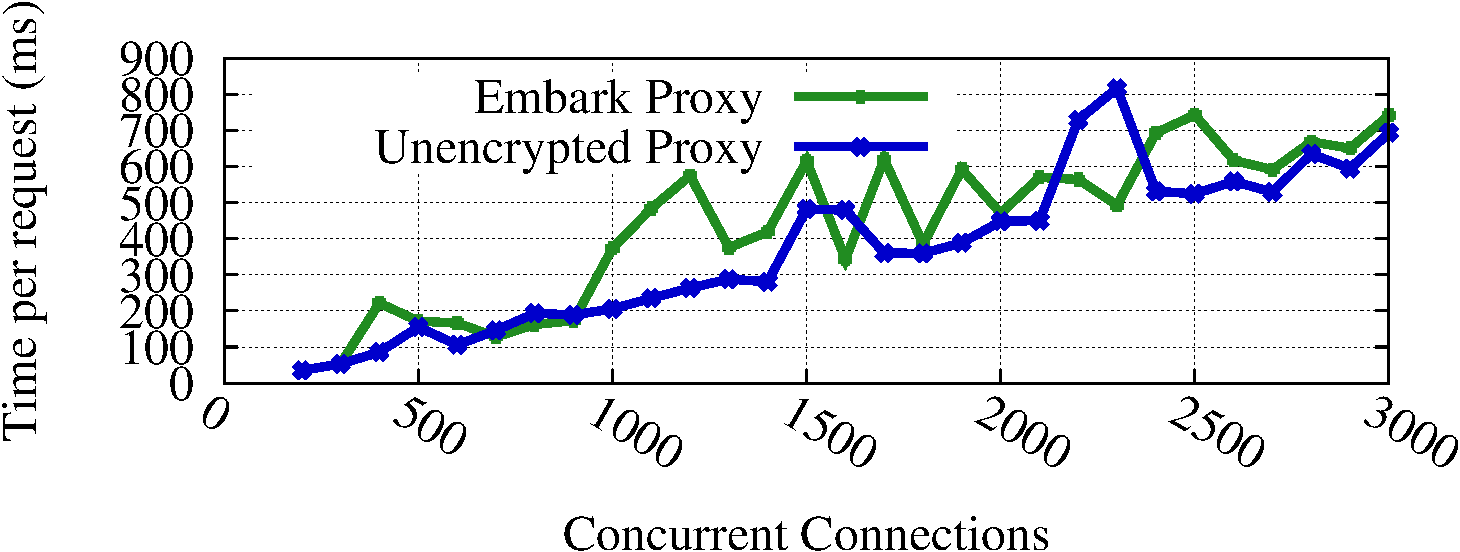
\includegraphics[width=3in]{fig/proxytime}
\caption{\label{fig:proxygraph} Access time per page against the number of concurrent connections at the proxy.}
\end{figure}

\noindent{\bf Proxy/Caching:} The throughput number shown in Table~\ref{tbl:appsxput} is not the typical metric used to measure proxy performance. A better metric for proxies is how many connections the proxy can handle concurrently, and what time-to-service it offers each client. In Figure~\ref{fig:proxygraph}, we plot time-to-service against the number of concurrent connections, and see that it is on average higher for \sys than the unencrypted proxy, by tens to hundreds of milliseconds per page.
This is not due to computation costs, but instead, due to the fact that the encrypted HTTP header values are transmitted on a different channel than the primary data connection.
The \sys proxy needs to synchronize between these two flows; this synchronization cost is what increases the time to service. 


\noindent{\bf Intrusion Detection:}
Our IDS is based on BlindBox~\cite{blindbox}. BlindBox incurs a substantial `setup cost' every time a client initiates a new connection. With \sys, however, the gateway and the cloud maintain one, long-term persistent connection. 
Hence, this setup cost is paid once when the gateway is initially configured. \sys also heurstically expands regular expressions in the rulesets into exact match strings. This results in two benefits:

\noindent{\it (1) End-to-end performance improves.} Where BlindBox incurs an initial handshake of 414s~\cite{blindbox} to open a new connection, clients under \sys never pay this cost; instead they perform a normal TCP or SSL handshake of only 3-5 RTTs. In our testbed, this amounts to between 30 and 100 ms, depending on the site and protocol -- an improvement of 4 orders of magnitude.

\noindent{\it (2) Security improves.} 
Using IDS rulesets from Snort, we converted regular expressions to exact match strings as discussed in \S\ref{sec:archblindbox}. With 10G memory, we were able to convert about half of all regular expressions to a finite number of exact match strings; the remainder resulted in too many possible states. 
We used two rulesets to evaluate this~\cite{emergingthreats, snort-community}. With the first ruleset BlindBox would resort to the lower security level for 33\% of rules, but \sys would only require this for 11.3\%.
With the second ruleset, BlindBox would use lower security for 58\% of rules, but \sys would only do so for 20.2\%.

\eat{
\begin{table}[h]
  \centering
  \small
  \begin{tabular}{l|c|c}
  %\begin{tabular}{p{1.75in}|p{.4in}|p{.4in}}
    {{\bf Rule Set}}&{\bf Exact Match}&{\bf Prob. Cause}\\
    \hline
    \hline
    BB: Community&67\%&100\%\\
    \hline
    MB: Community&88.7\%&100\%\\

    \hline
    \hline
    BB: Emerging Threats&42\%&100\%\\
    \hline
    MB: Emerging Threats&79.8\%&100\%\\
    \hline
  \end{tabular}
\end{table}
}


%!TEX root = mb.tex

\section{Related Work}
\label{sec:related}

\noindent{\bf Middlebox Outsourcing:}
APLOMB~\cite{aplomb} is a practical service for outsourcing enterprise's middleboxes to the cloud, which we discussed in detail in \S\ref{sec:overview}.

\noindent{\bf Data Confidentiality:}
Confidentiality of data in the cloud has been widely recognized as an important problem and researchers proposed solutions for software~\cite{Baumann:Haven}, web applications \cite{giffin:hails, Mylar},  filesystems~\cite{blaze:cfs, kallahalla:plutus, goh:sirius},  databases~\cite{popa:cryptdb},  and virtual machines~\cite{Zhang:CloudVisor}. 
CryptDB~\cite{popa:cryptdb} was one of the first practical systems to compute on encrypted data, but none of its encryption schemes or database system design apply to our network setting. 

Focusing on traffic processing, the most closely related work to \sys is BlindBox~\cite{blindbox}, discussed in \S\ref{sec:overview}.
mcTLS~\cite{mctls} proposed a protocol in which client and server can jointly authorize a middlebox to process certain portions of the encrypted traffic. Unlike \sys, the middlebox  gains access to unencrypted data and is still able to leak that data should it choose to do so. 

\noindent{\bf Trace Anonymization and Inference:}
Some systems which focus on {\it offline} processing allow some analysis over anonymized data \cite{Vern:Anonymize06, Vern:Anonymize03}; they are not suitable for online processing as is \sys.
Yamada et al~\cite{Yamada_IDS} show how one can perform some very limited processing on an SSL-encrypted packet by using only the size of data and the timing of packets, however they cannot perform analysis of the contents of connection data.

\noindent{\bf Encryption Schemes:}
\sys's RangeMatch scheme is similar to order preserving encryption schemes, but no existing scheme provided both the performance and security properties we required.
The order-preserving encryption~\cite{boldyreva:ope, popa:mope} used in CryptDB is 
 $>3000$ times slower than RangeMatch (\S\ref{sec:eval}); moreover, it leaks the order of the IP addresses encrypted, while RangeMatch protects this information. 
The encryption scheme of Boneh et al.~\cite{BonehRange} enables detecting if an encrypted value matches a range and provides a similar security guarantee to RangeMatch; but, it is orders of magnitude slower than the OPE schemes which are already 3000$\times$ slower than RangeMatch. 

%  mOPE unfortunately requires that the gateway and the service provider interact for a number of roundtrips (e.g., xxx in our experiments) which is too slow and requires additional setup for this interaction, and violates requirement~\ref{req:sec} or~\ref{req:injective}, and BCLO has weak security (leaking always the top half bits of the values encrypted and the order of IP addresses across different packets, thus violating requirement~\ref{req:sec}), is too slow, and not format-preserving. 

% HERE ARE A FEW USEFUL NOTES ABOUT HOW OUR DESIGN IS DIFFERENT FROM mOPE -- THERE IS SOME SIMILARITY DUE TO TREE AND ADJUST
% we do not readjust for encryption 
% - this is expensive, we do not leak data between two encryptions 
% The tree is stored at the gateway. The tree contains as nodes the ends of the intervals as opposed to all values encoded-- thus, the tree is much smaller. firewalls have on the order of thousands such rules, so the tree is not large. also store only ranges and not everything encoded, making it smaller and fit into the gateway, etc., they need adjustments when they encrypt too, etc. -- better point to related work for this
% Difference:
% we encode different values in the tree, have a different encryption algorithm, and create a much smaller tree that can be stored at the gateway. no roundtrips any more; they don't have the deterministic property
%store the tree at the gateway.
% This tree is stored at the gateway. The tree stores edges of the interval 
% one important point is that there are ciphertext updates only for rule changes and not for regular encryption








%!TEX root = mb.tex

\smallskip 

\section*{Acknowledgments}

We thank our shepherd, Srinivasan Seshan, and the anonymous reviewers for their thoughtful comments. We're also grateful to Dahlia Malkhi and Ittai Abraham from VMware Research for their valuable feedback on PrefixMatch.

\newpage
{\bibliographystyle{abbrv}
  \bibliography{related_work,cryptobib,rp,rp-str,rp-conf}}

  % That's all folks!
  \end{document}
